\chapter{Implementierung \& Test}
\label{chap: Implementierung und Test}
In diesem Kapitel wird beschrieben wie das im Kapitel \ref{chap: Konzept} vorgestellte Konzept in der Bibliothek \textit{gedcom7.js} implementiert wird. 

%========================================================================================
% SECTION: GEDCOM GRAMMATIK
%========================================================================================
% Reihenfolge Grammatik & Grammatik Generator??
\section{Gedcom Grammatik}
\label{sec: Implementierung - Gedcom Grammatik}
% zeigen wie eine Grammatik aussieht
% Zeigen wie der Postprocessor funktioniert (auch Ausschnitt von Lexer möglich)
% Problem mit Ambigious Grammar -> erklären was das Problem ist und wie gelöst wurde
\subsection{Gedcom7 Syntax in Nearley}
\label{subsec: Implementierung - Gedcom Grammatik - Gedcom7 Syntax in Nearley}
Da die Gedcom7- sowie die Nearley Syntax beide auf EBNF-Sprachkonzepten basieren, lässt sich die Gedcom7 Spezifikation ohne weiteres in eine Nearley Grammatik übersetzten. Um Nearley Regeln für eine \textit{Gedcom Line}\footnote{siehe \hyperref[sec: GEDCOM Version 7]{Kapitel GEDCOM Version 7}} zu definieren, können die folgenden Tokens für das Leerzeichen, den \textit{Cross-Reference Identifier} und die End-Of-Line Zeichenfolge in Form von regulären Ausdrücken definiert werden:
\\ \\
\begin{minipage}{1.0\textwidth} \small
	\begin{lstlisting}
		D    : /[ ]/
		Xref : /\@[A-Z0-9\_]+\@/	
		EOL  : /(?:\r\n?|\n)/
	\end{lstlisting}
	\captionof{lstlisting}{Tokens für eine Gedcom Line, definiert als regulärer Ausdruck }
	\label{lst: tokens gedcom line}
\end{minipage}
\\ \\
Diese regulären Ausdrücke werden in der Vorverarbeitungsphase vom Moo-Lexer verwendet, um zusammenhängende Zeichen zu Tokens zu gruppieren, die dann in der Nearley Grammatik über den Tokennamen mit einem vorangestellten \%-Zeichen angesprochen werden können. Soll nun die erste Line eines Family-Records geparsed werden, könnte dies mit der folgenden Nearley-Regel umgesetzt werden:
\\ \\
\begin{minipage}{1.0\textwidth} \small
	\begin{lstlisting}
		record_FAM -> "0"  %D  %Xref  %D  "FAM"  %EOL 
	\end{lstlisting}
	\captionof{lstlisting}{Nearley Regel zum parsen eines Family Records}
	\label{lst: nearley regel family record first line}
\end{minipage}
\\ \\
Diese Regel akzeptiert eine Line mit dem Level 0, einem syntaktisch korrekten Cross-Reference-Identifier, dem Tag \textit{FAM} gefolgt von einem EOL-Token. Getrennt werden die Bestandteile durch ein Leerzeichen. 


Sollen nun ebenfalls HUSB- und WIFE Structures als Substructures des Family Records akzeptiert werden, könnte die Nearley Grammatik wie folgt erweitert werden:
\\ \\
\begin{minipage}{1.0\textwidth} \small
	\begin{lstlisting}
		record_FAM
			-> "0"  %D  %Xref  %D  "FAM"  %EOL 
			|  record_FAM  record_FAM_Substructs:+
		
		record_FAM_Substructs 
			-> "1"  %D  "HUSB"  %D  %Xref  %EOL
			|  "1"  %D  "WIFE"  %D  %Xref  %EOL 
	\end{lstlisting}
	\captionof{lstlisting}{Nearley Regel zum parsen eines Family Records mit HUSB- und WIFE Substructures}
	\label{lst: nearley regel family record with husb and wife}
\end{minipage}
\\ \\
Auf diese Weise nimmt würde der Nearley Parser einen Family Record ohne Substructures und einen Family Record mit beliebig vielen Substructures (in diesem Fall HUSB- und WIFE Structures) als Eingabe akzeptieren. Sollen nun die weiteren Lines aus Listing \ref{lst: family record example} ebenfalls in die Grammatik aufgenommen werden, müssen Regeln für die Datentypen der Payloads des MARR-Events und der NCHI-Structure definiert werden. Die Anzahl der Kinder wird als  \textit{Integer} Datentyp kodiert, also ein Folge von Dezimalziffern. Nach der Gedcom7 Spezifikation dürfen \textit{Integer} Werte nicht leer sein und führende Nullen sind erlaubt, sollten aber vermieden werden. Eine Regel für den Datentyp \textit{Integer} kann also dargestellt werden als
\\ \\
\begin{minipage}{1.0\textwidth} \small
	\begin{lstlisting}
		digit    ->  [0-9]
		Integer  ->  digit:+
	\end{lstlisting}
	\captionof{lstlisting}{Nearley Regel für den Datentyp \textit{Integer}}
	\label{lst: nearley regel integer}
\end{minipage}
\\ \\ 
Für das MARR-Event, also die Hochzeit der Ehepartner der Familie, ist eine \textit{DATE Structure} zum Festhalten des Datums der Hochzeit hinterlegt. Dieses Datum wird mit dem Datentyp \textit{DateValue} kodiert, der im Gegensatz zum \textit{Integer} wesentlich mehr Regeln umfasst. Ein \textit{DateValue} kann auf vier verschiedene Weisen dargestellt sein:
\begin{enumerate}
	\item \textit{date}: Ein mehr oder weniger genau spezifiziertes Datum, z.B. ``JULIAN 13 MAR 1998 BCE''
	\item \textit{datePeriod}: Ein Zeitintervall, dass von einem Startdatum bis zu einem Enddatum angegeben wird, z.B. ``FROM 15 FEB 2001 TO 23 MAR 2001''
	\item \textit{dateRange}: Ein ungenaueres Zeitintervall, bei dem nur Grenzen angegeben werden, z.B. ``BET 15 FEB 2001 AND 23 MAR 2001''
	\item \textit{dateApprox}: Eine Schätzung des Datums (ABT x: genaues Datum unbekannt, aber nahe x), z.B. ``ABT 15 FEB 2001''
\end{enumerate}
Diese Zusammenhänge ergeben die folgenden Nearley Regeln für die Definition des Datentyps \textit{DateValue}:
\\ \\
\begin{minipage}{1.0\textwidth} \small
	\begin{lstlisting}
		DateValue   ->  (date | DatePeriod | dateRange | dateApprox):?
		
		date        ->  (calendar  D):?  
						((day  D):?  month  D):?  
						year  
						(D  epoch):?
		datePeriod  ->  ("FROM"  D  date  D):?  "TO"  D  date
		dateApprox  ->  ("ABT" | "CAL" | "EST")  D  date 
		dateRange   ->  "BET"  D  date  D  "AND"  D  date  
					|   "AFT"  D  date  
					|   "BEF"  D  date 
		
		calendar ->  "GREGORIAN" | "JULIAN" | "FRENCH_R" | "HEBREW"
		day      ->  Integer  
		year 	 ->  Integer
		month    ->  Tag
		epoch    ->  "BCE" | Tag
		
		Tag 	 ->  upperCaseLetter  |  digit  |  underscore 
	\end{lstlisting}
	\captionof{lstlisting}{Nearley Regel für den Datentyp \textit{DateValue}}
	\label{lst: nearley regel date}
\end{minipage}
\\ \\ 
Werden all diese Regeln zusammengefasst lässt sich die folgende Grammatik definieren, die den Family Record aus Listing \ref{lst: family record example} als Eingabe akzeptiert:
\\ \\
\begin{minipage}{1.0\textwidth} \small
	\begin{lstlisting}
		record_FAM_Substructs
			-> "0"  %D  %Xref  %D  "FAM"  %EOL 
			|  record_FAM  record_FAM_Substructs:+
		
		record_FAM_Substructs 
			-> "1"  %D  "HUSB"  %D  %Xref  %EOL
			|  "1"  %D  "WIFE"  %D  %Xref  %EOL 
			|  "1"  %D  "NCHI"  %D  Integer  %EOL 
			|  structure_MARR 
		
		structure_MARR
			-> "1"  %D  "MARR" %EOL
			|  structure_MARR  
		
		structure_DATE
			-> "2" %D  "DATE"  %D  DateValue  %EOL
	\end{lstlisting}
	\captionof{lstlisting}{Nearley Grammatik für den Family Record aus Listing \ref{lst: family record example}}
	\label{lst: vollständige nearley grammatik family record}
\end{minipage}
\\ \\ 
Mit diesem Vorgehen können Nearley Regeln für alle Datentypen, Structures und Records definiert werden, die zu einer Grammatik für die Syntaxüberprüfung von Gedcom7 Dateinen zusammengesetzt werden können.


\subsection{Nearley Postprozessor}
\label{subsec: Implementierung - Gedcom Grammatik - Nearley Postprozessoren}
Der Nearley Postprozessor für die Bibliothek \textit{gedcom7.js} enthält 3 Funktionen: 

\vspace{1em}
\textsc{\textbf{joinAndUnpackAll()}:} \vspace{0.5em} \\
Wie in Abschnitt \ref{subsec: Konzept - Gedcom Grammatik - Pre- und Postprozessor} beschrieben, überführt ein \textit{Nearley-Parser} jedes Zeichen, das mit einer Regel übereinstimmt, in ein Array. Bei komplexeren Grammatiken wie der Gedcom7 Spezifikation führt dies dazu, dass sehr viele Arrays innereinander verschachtelt werden, sodass schnell hohe Verschatlungsgrade erreicht werden. Ein Beispiel hierfür wäre der in Abschnitt \ref{subsec: Implementierung - Gedcom Grammatik - Gedcom7 Syntax in Nearley} definierte Datentyp \textit{DateValue}. Hier würde jeder Bestandteil eines DateValues in ein eigenes Array verschachtelt werden. Wird beispielsweise das Datum 
\begin{center}
	13 MAR 1998 BCE
\end{center}
ohne Postprozessoren verarbeitet, wird das Array
\begin{center}
	[13, , [MAR, , [1998, , [BCE, , ]]]]
\end{center}
zurückgegeben, dass eine Weiterverarbeitung sehr umständlich macht. Daher wird der Postprozessor \textsc{joinAndUnpackAll()} implementiert, der über die JavaScript Funktion \textit{flat()} alle Elemente des Arrays rekursiv verkettet und anschließend über die Funktion \textit{join()} zu einer Zeichenkette zusammenfügt. Wird dieser Postprozessor einem Datentyp wie \textit{DateValue} zugewiesen, wird jedes syntaktisch korrekte Datum als Zeichenkette zurückgegeben und kann so direkt als LineValue für die weitere Verarbeitung verwendet werden. Die in Listing \ref{lst: nearley regel date} definierte Regel würde sich ergeben zu
\\ \\
\begin{minipage}{1.0\textwidth} \small
	\begin{lstlisting}
		DateValue   
			->  (date | DatePeriod | dateRange | dateApprox):?
				
	\end{lstlisting}
	\captionof{lstlisting}{Erweiterung der Nearley Regel für den Datentyp \textit{DateValue}}
	\label{lst: nearley regel date mit postprozessor}
\end{minipage}
\\ \\

\vspace{1em}
\textsc{\textbf{createStructure()}:} \vspace{0.5em} \\
Der Postprozessor \textsc{createStructure()} wird verwendet, um die gelesene Line mit Structure Informationen anzureichern. In der Nearley Regel wird die Line selbst, der Typ und die in der Gedcom7 Spezifikation definierte URI der Line und die Structures bei denen eine Kardinalitätsüberprüfung notwendig ist an den Postprozessor übergeben. Für den in Listing \ref{lst: vollständige nearley grammatik family record} Family Record ergibt sich der Postprozessoraufruf wie folgt:
\\ \\
\begin{minipage}{1.0\textwidth} \small
	\begin{lstlisting}
		record_FAM
			-> "0"  %D  %Xref  %D  "FAM"  %EOL
			
	\end{lstlisting}
	\captionof{lstlisting}{Nearley Regel zum parsen eines Family Records mit Postprozessor}
	\label{lst: nearley regel family record mit postprozessor}
\end{minipage}
\\ \\
Im Parameter \textit{checkCardinalityOf} werden die URIs alle Structures angegeben, bei denen eine Kardinalitätsüberprüfung notwendig ist und die in der Gedcom7 Spezifikation definierte Kardinalität als Wert zugewiesen. Kardinalitätsüberprüfungen sind bei allen Substructures erforderlich, die für die SUperstructure als notwendig definiert wurden (1:1 und 1:M) oder für die eine Maximale Anzahl festgelegt ist (also 0:1 und 1:1). In der Funktion \textsc{createStructure()} werden alle Informationen abhängig vom übergebenen Type zusammengefasst und als JavaScript Objekt an den Parser zurückgegeben. Für einen Family Record ergibt sich die Funktion zu:
\\ \\
\begin{minipage}{1.0\textwidth} \small
	\begin{lstlisting}
	createStructure: (params) => {
		// create line object depending on type of line
		let lineObject = {};
		lineObject = { 
			level: line[0], 
			xref: line[2], 
			tag: line[4], 
			lineVal: '', 
			EOL: line[5] 
		};
		
		// return data object with structure information
		return {
			uri: params.uri,
			line: lineObject,
			type: params.type,
			lineValType: params.lineValType || null,
			superstructFound: false,
			substructs: [],
			checkCardinalityOf: params.checkCardinalityOf
		};
	}
	\end{lstlisting}
	\captionof{lstlisting}{Funktion \textsc{createStructure()} für einen Family Record}
	\label{lst: createStructure für Family Record}
\end{minipage}
\\ \\

\vspace{1em}
\textsc{\textbf{addSubstructure()}:} \vspace{0.5em} \\
Die zusammengesetzte Regel ergibt sich zu 
\\ \\
\begin{minipage}{1.0\textwidth} \small
	\begin{lstlisting}
		record_FAM
			-> "0"  %D  %Xref  %D  "FAM"  %EOL
			
	\end{lstlisting}
	\captionof{lstlisting}{Vollständige Nearley Regel zum parsen eines Family Records mit Substructures}
	\label{lst: nearley regel family record mit postprozessor und substructs}
\end{minipage}
\\ \\

%========================================================================================
% SECTION: GRAMMATIK GENERATOR
%========================================================================================
\section{Grammatik Generator}
\label{sec: Implementierung - Grammatik Generator}
Der in Abschnitt \ref{sec: Konzept - Grammatik Generator} vorgestellte Grammatik Generator wird über die Klasse \textsc{GrammarGenerator}, wie in Abbildung \ref{fig: UML Klassendiagramm GrammarGenerator} dargestellt, implementiert. Über die Klassenmethode \textit{build(path)} kann eine Instanz von \textsc{GrammarGenerator} erstellt werden, der die Gedcom Grammatik an dem mit dem Parameter \textit{path} spezifizierten Pfad erzeugt. Bei der Instanzerzeugung wird im ersten Schritt der Nearley-Header, der in der Nearley Datei \textit{NearleyHeader.ne} spezifiziert ist, eingelesen und als Instanzvariable in Form einer Zeichenkette gespeichert. Dieser Nearley-Header stellt den obersten Eintrag jeder Nearley-Datei dar, die vom \textsc{GrammarGenerator} erzeugt wird und enthält die Include-Statements für Datentypen, Postprozessoren, etc. und den Aufruf des Moo-Lexers. Anschließend werden die Gedcom Grammatik Definition, die in Form von JavaScript Objekten gespeichert sind, gelesen und gespeichert. Anschließend kann diese Gedcom Grammatik Definition mit der Funktion \textit{generateGrammar()} in Nearley-Dateien überführt werden, die dann zu Nearley Parsern kompiliert werden können. In den folgenden Kapitel wird auf diese Schritte im Detail eingegangen.
\begin{figure}[h]
	\centering
	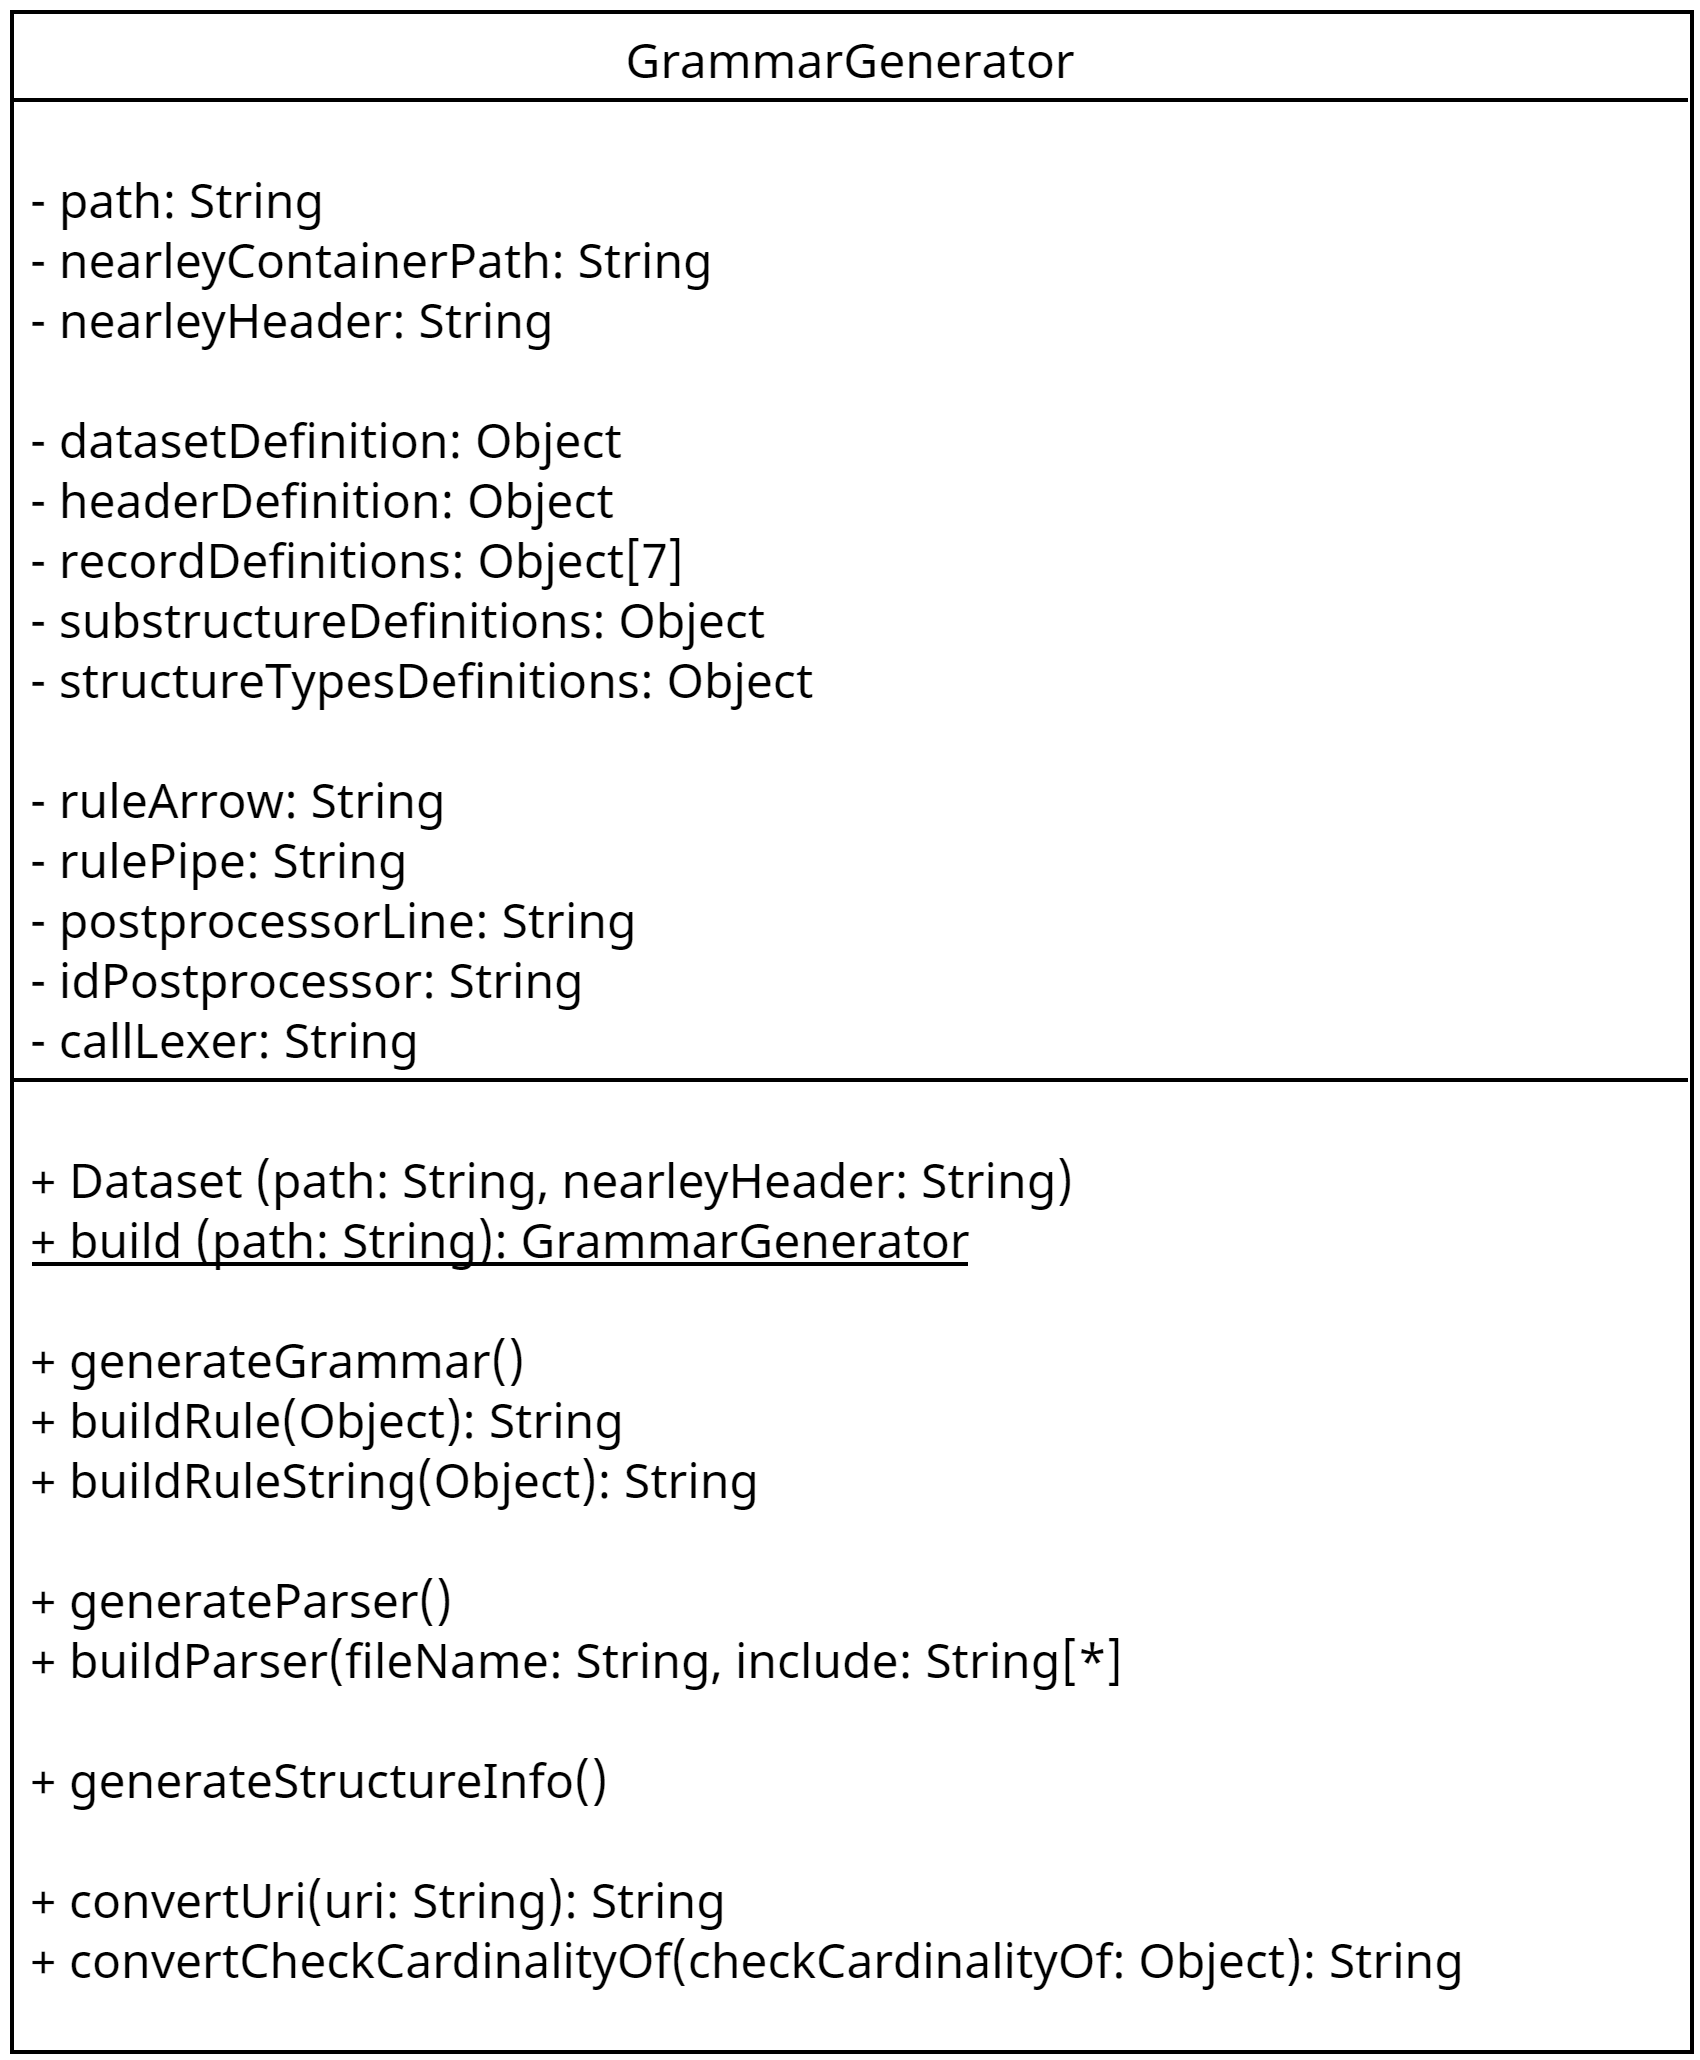
\includegraphics[width=1\textwidth]{images/UML_Class_GrammarGenerator.png}
	\caption{UML Klassendiagramm GrammarGenerator}
	\label{fig: UML Klassendiagramm GrammarGenerator}
\end{figure}

\subsection{Definition der Grammatik}
\label{subsec: Implementierung - Grammatik Generator - Definition der Grammatik}
Die Definition der Gedcom Grammatik erfolgt in Form von JavaScript Objekten. Für jede Structure, die in der Gedcom7 Spezifikation definiert ist, wird eine Grammatik Definition erstellt. Folgende Parameter sind in diesen Objekten hinterlegt:
\bgroup
\def\arraystretch{1.5}%  1 is the default, change whatever you need
\setlength{\tabcolsep}{18pt}
\begin{tabular}{|p{2cm}|p{10cm}|}
	\hline
	\textbf{URI} & Die in der Gedcom7 Spezifikation für diese Structure hinterlegte URI. \\
	\hline
	\textbf{lineType} & Der Typ der Line einer Structure (hier wird beispielsweise hinterlegt, ob die Structure einen Cross-Reference-Identifier enthält oder auf andere Structuren verweisen darf). \\
	\hline
	\textbf{Info} & In der Info wird ein Informationstext zu jeder Strucutre hinterlegt. Dieser kann verwendet werden um bei Verwendung der Bibliothek dem Benutzer Informationen über die Bedeutung der Structures zukommen zu lassen.\\
	\hline
	\textbf{Level} & Die Levels unter denen die Structure in einer Gedcom7 Datei auftauchen kann.\\
	\hline
	\textbf{Tag} & Der in der Gedcom7 Spezifikation definierte Tag der Structure.\\
	\hline
	\textbf{Substructs} & Alle Structures, die als Substructure für eine Structure auftauchen können, inkl. der Kardinalität dieser.\\
	\hline
\end{tabular}
\egroup
\\ \\
Die Definition für einen Family Record sieht wie folgt aus. Anders als bei den Beispielen aus Abschnitt \ref{sec: Implementierung - Gedcom Grammatik} bei denen nur ein Teil der Substructures betrachtet wurde, handelt es sich hierbei um eine vollständige Definition:
\\ \\
\begin{minipage}{1.0\textwidth} \small
	\begin{lstlisting}
		{
			uri: 'g7:record-FAM',
			lineType: lineTypes.FAM_RECORD,
			info: 'Structure Info coming soon!',
			level: [0],
			tag: 'FAM',
			substructs: {
				'g7:RESN': '0:1',
				FAMILY_ATTRIBUTE_STRUCTURE: '0:M',
				FAMILY_EVENT_STRUCTURE: '0:M',
				NON_EVENT_STRUCTURE: '0:M',
				'g7:FAM-HUSB': '0:1',
				'g7:FAM-WIFE': '0:1',
				'g7:CHIL': '0:M',
				ASSOCIATION_STRUCTURE: '0:M',
				'g7:SUBM': '0:M',
				LDS_SPOUSE_SEALING: '0:M',
				IDENTIFIER_STRUCTURE: '0:M',
				NOTE_STRUCTURE: '0:M',
				SOURCE_CITATION: '0:M',
				MULTIMEDIA_LINK: '0:M',
				CHANGE_DATE: '0:1',
				CREATION_DATE: '0:1'
			}
		}
	\end{lstlisting}
	\captionof{lstlisting}{Grammatik Definition eines Family Records}
	\label{lst: Grammatik Definition Family}
\end{minipage}
\\ \\

\subsection{Grammatikgenerierung mit generateGrammar()}
\label{subsec: Implementierung - Grammatik Generator - generateGrammar}
Nach dem in Abschnitt \ref{subsec: Implementierung - Grammatik Generator - Definition der Grammatik} beschriebenen Vorgehen werden Grammatik Definitionen für alle Structuretypes, Substructures und Records, sowie für das gesamte Dataset erstellt. Mit der Funktion \textit{generateGrammar()} werden diese eingelesen, in eine nearley-konforme Zeichenkette konvertiert und anschließend in Form einer Nearley Datei (.ne) gespeichert. Die Regeln werden mit der Funktion \textit{buildRuleString()} erzeugt und mit den in der Klasse \textsc{GrammarGenerator} definierten Building-Konstanten zusammengefügt. Ein Beispiel für eine solche Konstante ist der \textit{ruleArrow} der zur Definition einer Regel verwendet wird und als Zeichenkette ''\escape{n}\escape{t} \textendash\textgreater`` kodiert ist. Die so erzeugten Nearley Dateien sind somit einfach lesbar und liegen in der in Abschnitt \ref{subsec: Implementierung - Gedcom Grammatik - Gedcom7 Syntax in Nearley} Form vor. Alle so erstellten Nearley Dateien werden im mit \textit{path} spezifizierten Pfad im Verzeichnis ''\textit{path/nearley/}`` abgelegt.

\subsection{Parsergenerierung mit generateParser()}
\label{subsec: Implementierung - Grammatik Generator - generateParser}
Mit der Funktion \textit{generateParser()} werden die Nearley Grammatiken für alle Records und das gesamte Dataset zu Nearley Parsern kompiliert. Dazu stellt Nearley die Funktion 
\begin{center}
	nearleyc  \textit{inputPath} -o \textit{outputPath}
\end{center}
bereit, mit eine Nearley Datei eingelesen und im spezifizierten Pfad kompiliert werden kann. Das Erstellen von Parsern für die Records ist notwendig, da die Nearley Parser für die Syntaxüberprüfung nach Änderung eines Records verwendet werden. Würde nur ein allgemeiner Dataset-Parser erstellt werden, müsste nach jeder Änderung das komplette Dataset überprüft werden, obwohl nur ein Record verändert wurde. 

Im ersten Schritt der Funktion \textit{generateParser()} werden die Include-Statements vorbereitet, die z.B. die Definition der Datentypen enthalten. Anschließend wird für die Record- und Dataset-Grammatiken die Funktion \textit{buildParser()} aufgerufen, die in Listing \ref{lst: GrammarGenerator Funktion buildParser()} dargestellt ist. Hier werden die mit \textit{generateGrammar()} erzeugte Grammatik, die Include-Statements und der Nearley Header in einer Container Datei \textit{NearleyContainer.ne} zusammengefügt. Diese Container Datei wird anschließend zu dem entsprechenden Parser kompiliert und im mit \textit{path} spezifizierten Pfad im Verzeichnis ''\textit{path/parser/}`` abgelegt.
\\ \\
\begin{minipage}{1.0\textwidth} \small
	\begin{lstlisting}
	// build nearley-file with include statements and NearleyHeader inside of NearleyContainer.ne file and compile it to a nearley parser
	async buildParser (fileName, include) {
		// string representation of the grammar to be compiled
		let fileStr = '';
		
		// add given include statements
		for (const file of include) {
			fileStr += `@include "../grammar/nearley/${file}"\n`;
		}
		
		// add nearley header
		fileStr += this.nearleyHeader;
		
		// overwrite content of NearleyContainer file
		await fs.writeFile(this.nearleyContainerPath, fileStr);
		
		// read grammar of given file
		const grammar = await fs.readFile(`${this.path}nearley/${fileName}.ne`, { encoding: 'utf8' });
		
		// append grammar to NearleyContainer file
		fs.appendFile(this.nearleyContainerPath, grammar);
		
		// compile composed NearleyContainer.ne file to nearley parser
		await exec(`npx nearleyc ${this.nearleyContainerPath} -o ${this.path}parser/${fileName}Parser.js`);
	}
	\end{lstlisting}
	\captionof{lstlisting}{Funktion buildParser() des Grammatik Generators}
	\label{lst: GrammarGenerator Funktion buildParser()}
\end{minipage}
\\ \\

%========================================================================================
% SECTION: GEDCOM STRUKTUR
%========================================================================================
\section{Gedcom Struktur}
\label{sec: Implementierung - Gedcom Struktur}
Die Struktur einer Gedcom7 Datei wird in der Bibliothek \textit{gedcom7.js} mit Hilfe der Klasse \textsc{Dataset} abgebildet, die alle Gedcom Structures verwaltet, die in Form der gleichnamigen Klasse \textsc{Structure} verwaltet werden. Structures werden in \textit{gedcom7.js} entweder als allgemeine Instanz der Klasse \textsc{Structure} (z.B. eine HUSB-Structure), als \textsc{Record} (z.B. ein Family Record) oder als \textsc{Datatype Structure} (z.B. eine DATE-Structure) repräsentiert. 

\subsection{Klasse \textsc{Structure}}
\label{subsec: Implementierung - Gedcom Struktur - Klasse Structure}
Die Klasse \textsc{Structure} ist die Überklasse aller Klassen zur Structure-Verwaltung, d.h. Records und Datatyp Structures erben alle Methoden und Eigenschaften von \textsc{Structure}. Diese Methoden und Eigenschaften sind in Abbildung \ref{fig: UML Klassendiagramm Structure} abgebildet. 

\begin{figure}[h]
	\centering
	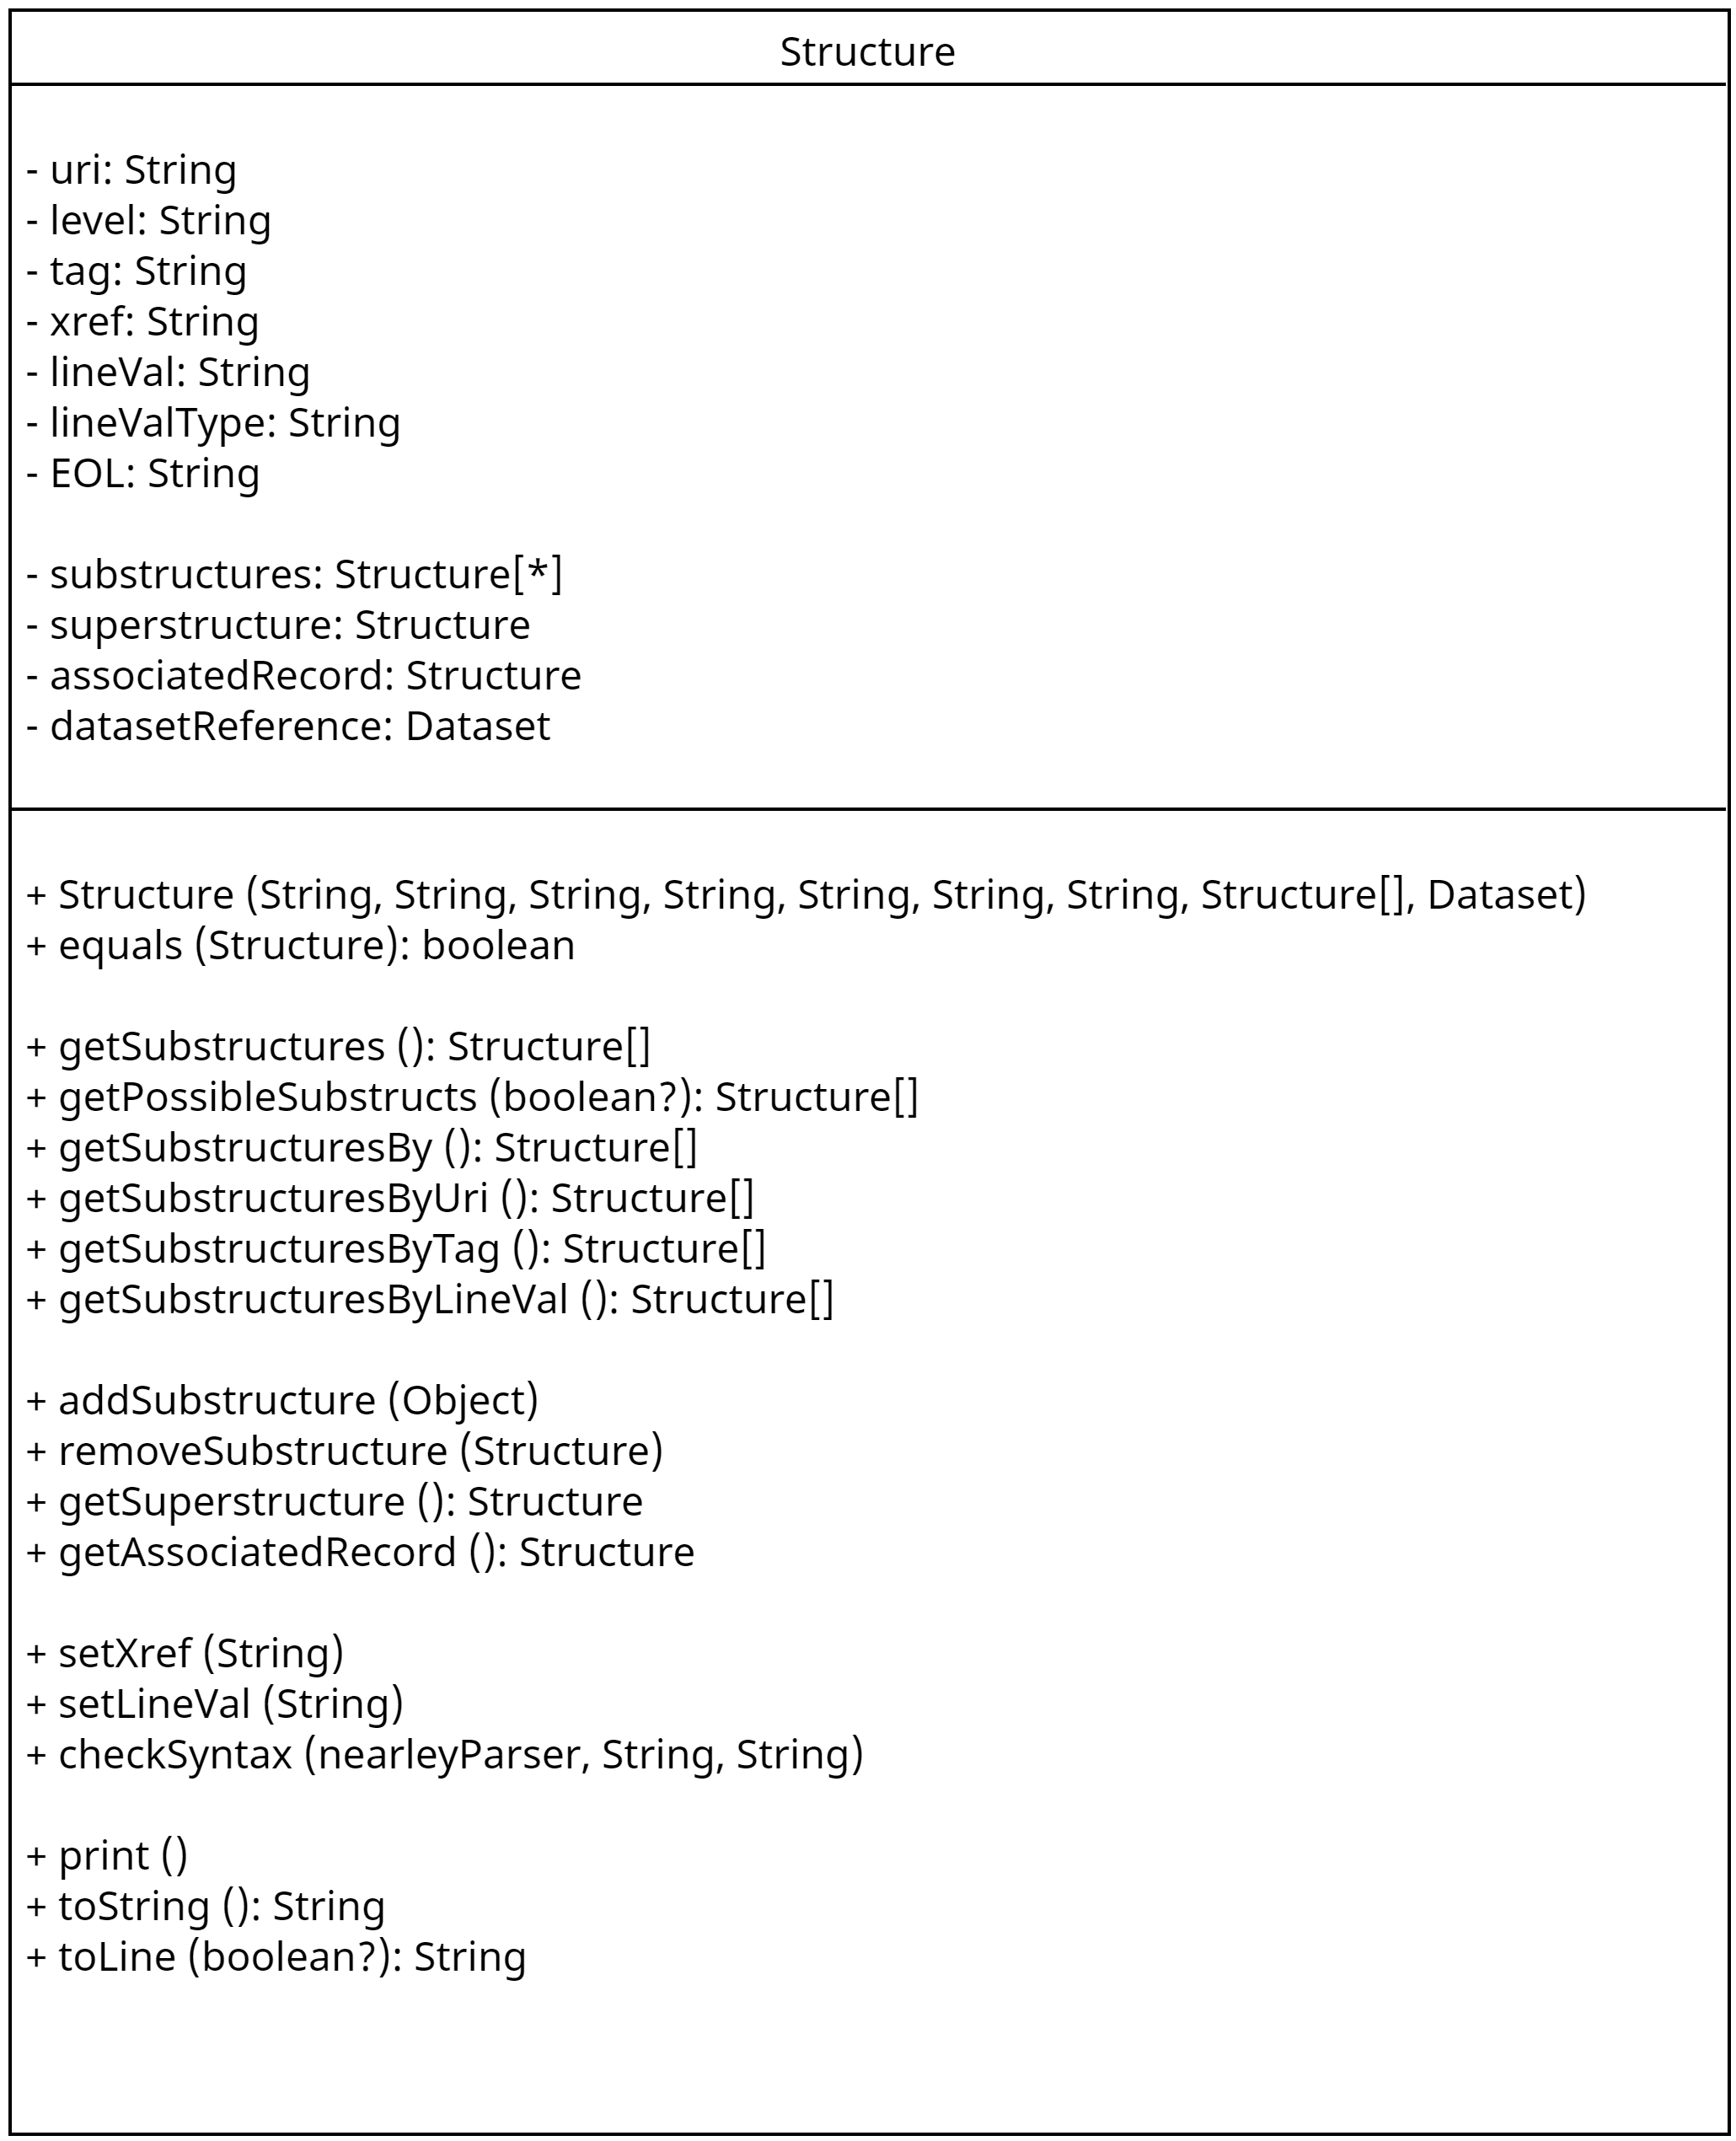
\includegraphics[width=1\textwidth]{images/UML_Class_Structure.png}
	\caption{UML Klassendiagramm Structure}
	\label{fig: UML Klassendiagramm Structure}
\end{figure}

Eine Instanz der Klasse \textsc{Structure} hält alle Informationen über eine Line bereit (URI, Level, Tag, Xref, lineValue, Typ des LineValues, EOL-Zeichen). Außerdem werden Referenzen zu allen Substructures, der Superstructure, dem Record mit dem die Structure assoziiert wird, sowie zum Dataset in dem die Structure enthalten ist bereitgestellt. Außerdem übernimmt die Klasse \textsc{Structure} vier zentrale Aufgaben zur Verwaltung von Gedcom7 Informationen, die von der Klasse \textsc{Dataset} angestoßen werden können:

\vspace{1em}
\textbf{1. Finden von Substructures} \vspace{0.5em} \\
Eine der wichtigsten Aufgaben der Klasse \textsc{Structure} ist es, eigene Substructures zu suchen und zu finden. Dazu werden die Methoden \textit{getSubstructuresByUri}, \textit{getSubstructuresByTag} und \textit{getSubstructuresByLineVal} bereitgestellt, die alle Substructures zurückgeben, die einem Suchkriterium genügen, das abhängig von der Methode eine Gedcom7 URI, ein Gedcom7 Tag oder einen LineValue darstellen. Über den Parameter \textit{recursive} kann spezifiziert werden, ob nur direkte Substructures (also mit einem um $1$ inkrementierten Level) gesucht werden sollen oder ob ebenfalls alle Substructures von Substructures rekursiv durchsucht werden sollen. Sollen einfach alle Substructures einer Structure ohne Suchkriterium zurückgegeben werden, kann die Methode \textit{getSubstructures} verwendet werden.


In vielen Anwendungsfällen kann es zudem von Interesse sein, welche Structures als Substructure in Frage kommen (also welche Structures in der Gedcom7 Spezifikation als potentitelle Substructures definiert sind). Ein Beispiel hierfür wäre ein Benutzer, der einen Family Record verwaltet und herausfinden möchte, welche weiteren Informationen angegeben werden können. FÜr diesen Fall wird die Methode \textit{getPossibleSubstructs} bereitgestellt, die die Gedcom7 URIs aller Structures zurückgibt, die als Substructure auftreten können. Über den boolschen Parameter \textit{checkCardinalityFlag} kann spezifiziert werden, ob die Kardinalität überprüft werden soll, d.h. ob nur diejenigen URIs bereitgestellt werden sollen, die beim Hinzufügen nicht zu einem CardinalityError führen. 

\vspace{1em}
\textbf{2. Hinzufügen und Entfernen von Substructures} \vspace{0.5em} \\
Die Klasse \textsc{Structure} stellt die Methode \textit{addSubstructure} zur Verfügung, um einer Instanz der Klasse eine Substructure hinzuzufügen (siehe Abbildung \ref{fig: UML Aktivität addSubstructure}). Dazu werden alle nötigen Informationen über die Substructure als Parameter \textit{StructureParameter} übergeben. In der Methode werden diese Informationen extrahiert und auf Basis dessen eine neue Instanz der Klasse \textsc{Structure} erstellt. Dieses Object wird in das Dataset eingefügt indem alle nötigen Referenzen angepasst werden und das Object Teil der Gedcom Struktur wird. Anschließend wird die Syntax des Records überprüft, in den die neue Structure eingefügt wurde um zu überprüfen, ob immernoch ein Gedcom7 konformes Dataset vorliegt. Ist dies der Fall wird im Dataset überprüft, ob undefinierte Cross-Reference-Identifier vorliegen. 


Falls eine dieser Überprüfungen fehlschlägt, wird die Substructure über die Methode \textit{removeSubstructure} aus dem Dataset entfernt, indem die gleichnamige Methode der Klasse \textsc{Dataset} aufgerufen wird (siehe Abschnitt \ref{subsec: Implementierung - Gedcom Struktur - Klasse Dataset}).
\begin{figure}[h]
	\centering
	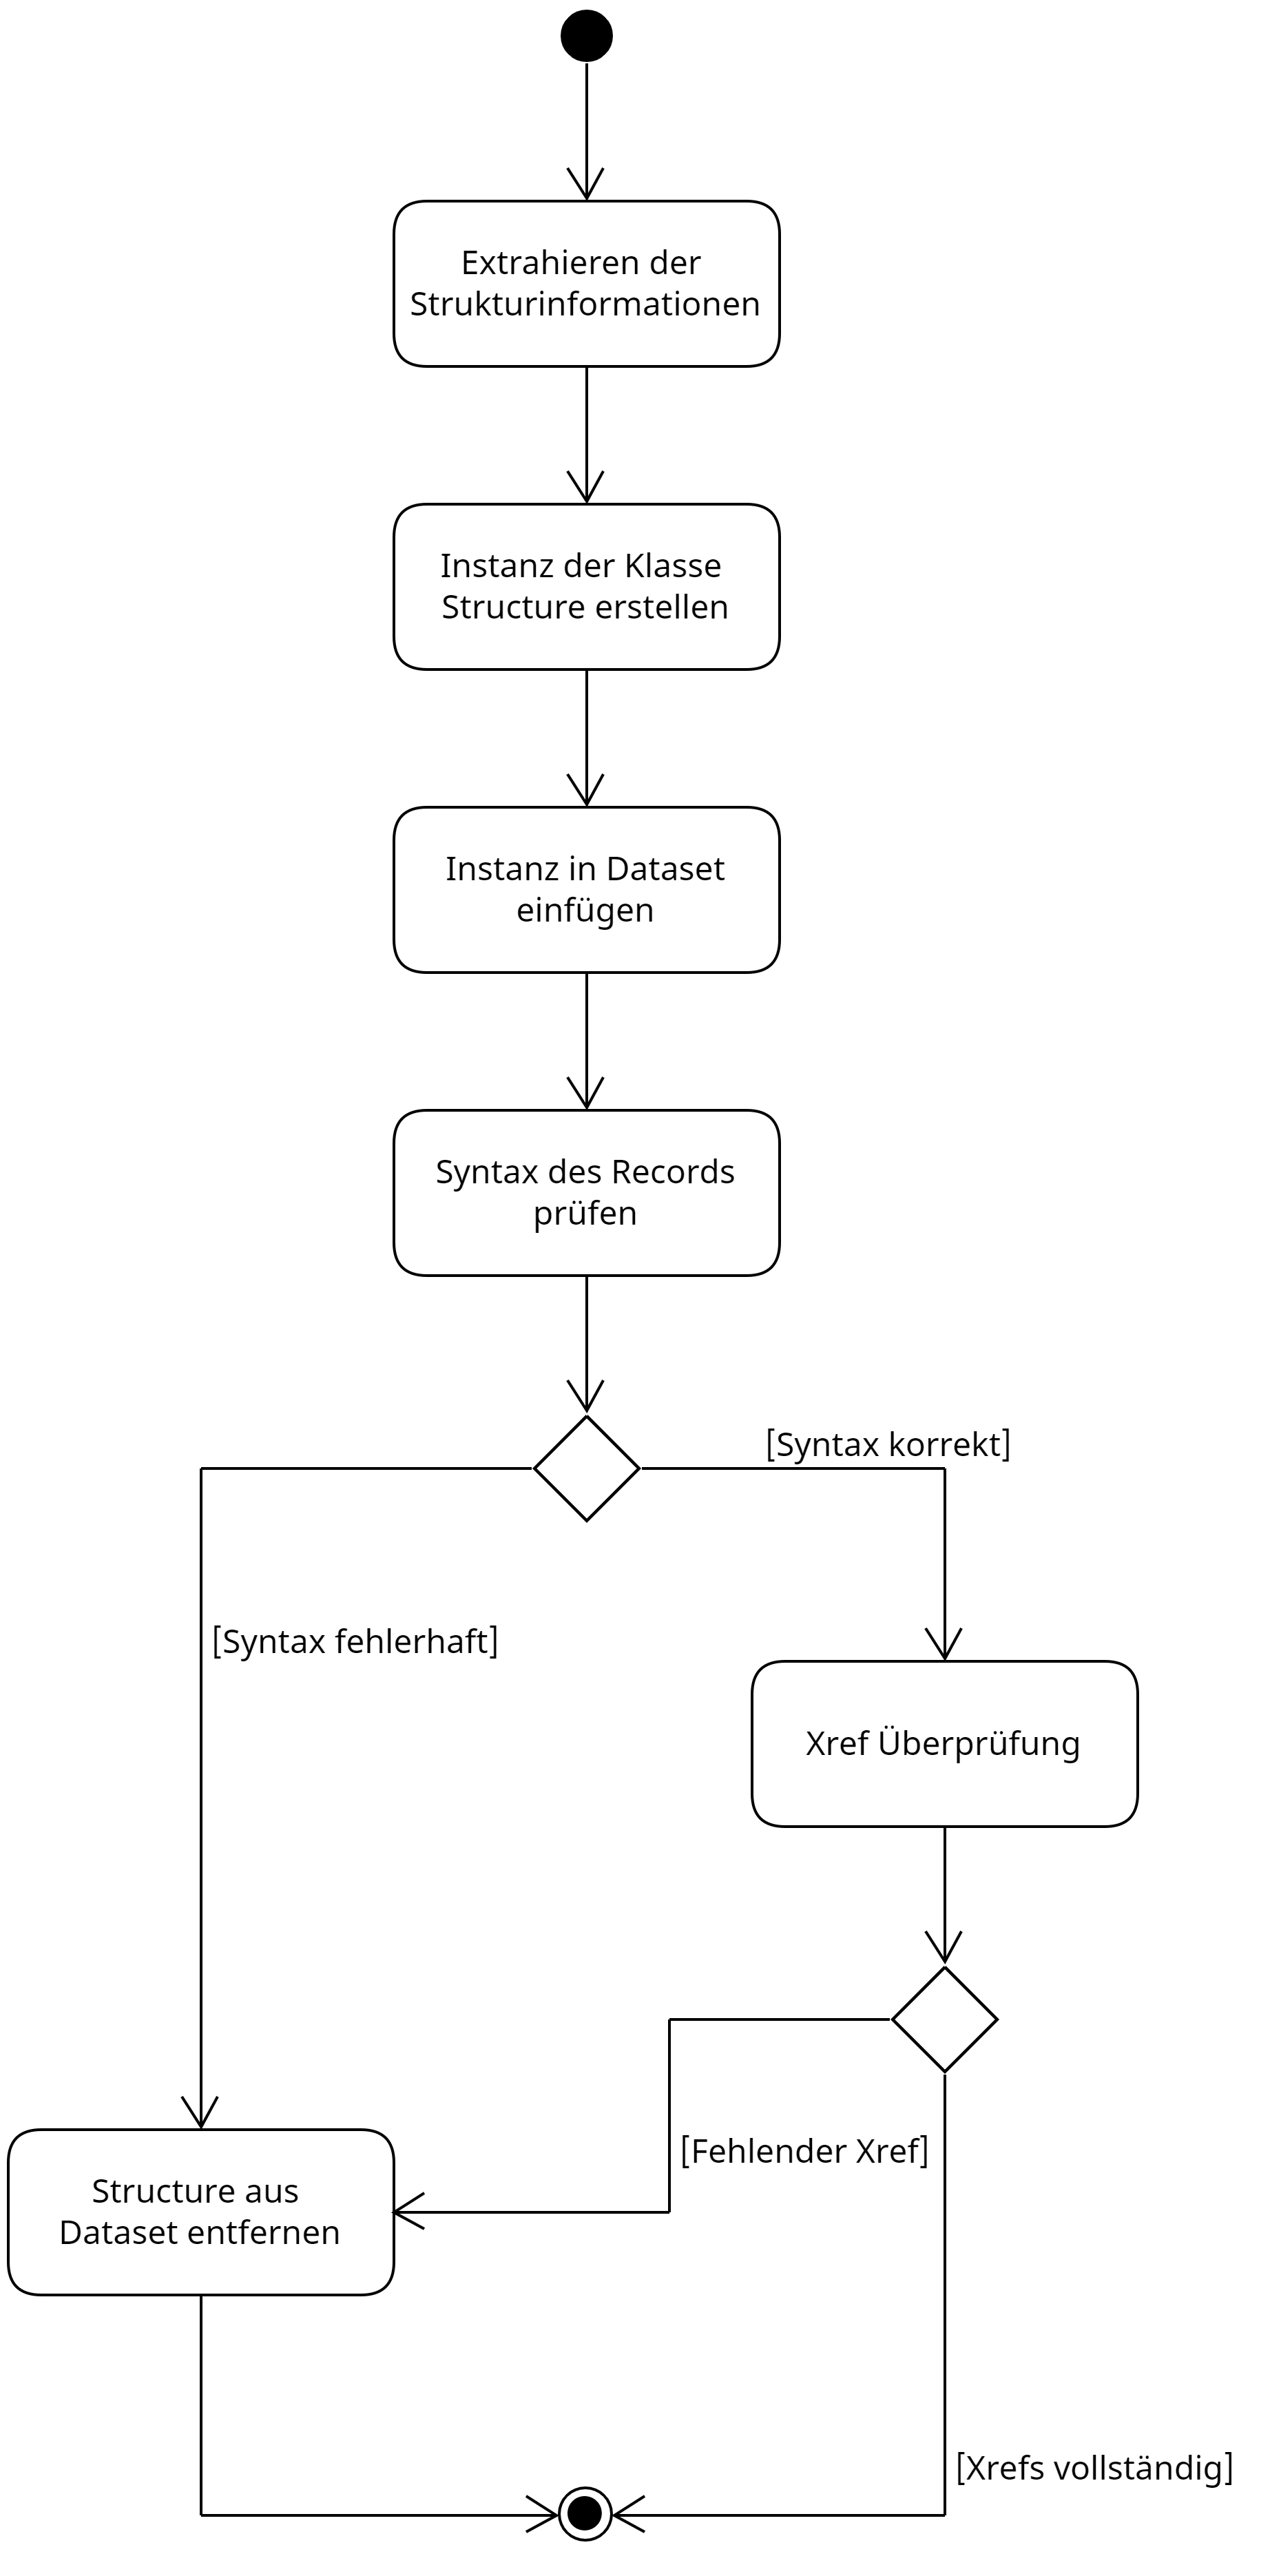
\includegraphics[width=0.5\textwidth]{images/UML_Activity_AddSubstruct.png}
	\caption{UML Aktivitätsdiagramm der Methode \textit{addSubstructure}}
	\label{fig: UML Aktivität addSubstructure}
\end{figure}

\vspace{1em}
\textbf{3. Ändern des LineValues} \vspace{0.5em} \\
Der LineValue einer Instanz der Klasse \textsc{Structure} kann über die Methode \textit{setLineVal} verändert werden (siehe Abbildung \ref{fig: UML Aktivität setLineVal}). Die Eigenschaft \textit{lineVal} des \textsc{Structure} Objekts wird auf den als Parameter übergebenen Wert gesetzt und anschließend wird die Syntax des entsprechenden Records überprüft, um zu kontrollieren, dass der neue LineValue syntaktisch korrekt ist.
Handelt es sich um eine Structure, die einen LineValue des Typs \textit{Xref}\footnote{Ein Beispiel hierfür wäre die HUSB-Structure, die auf einen Individual Record verweist.} besitzt, also auf eine andere Structure verweist, muss ebenfalls \textit{Xref-Map} des Datasets aktualisiert werden. In dieser Map werden alle Verweise über Cross-Reference-Identifier, die im Dataset vorkommen, verwaltet. Werden nach der Veränderung des LineValues ein Syntaxfehler oder undefinierte Cross-Reference-Identifier gefunden, muss der LineValue auf den Ursprungswert zurückgesetzt werden. 

Da auch ein leerer LineValue syntaktisch korrekt sein kann, wird im letzten Schritt das Dataset nach leeren Structures durchsucht, die dann entfernt werden. Ein Beispiel hierfür wäre die MARR-Structure aus dem Family Record in Listing \ref{lst: family record example}. Würde hier der DATE-Structure ein leerer Wert zugewiesen werden, würde dies in der Structure
\begin{center}
	1 MARR\\
	2 DATE
\end{center}
resultieren. Diese Structure enthält keinerlei Informationen und kann daher entfernt werden.
 
\begin{figure}[h]
	\centering
	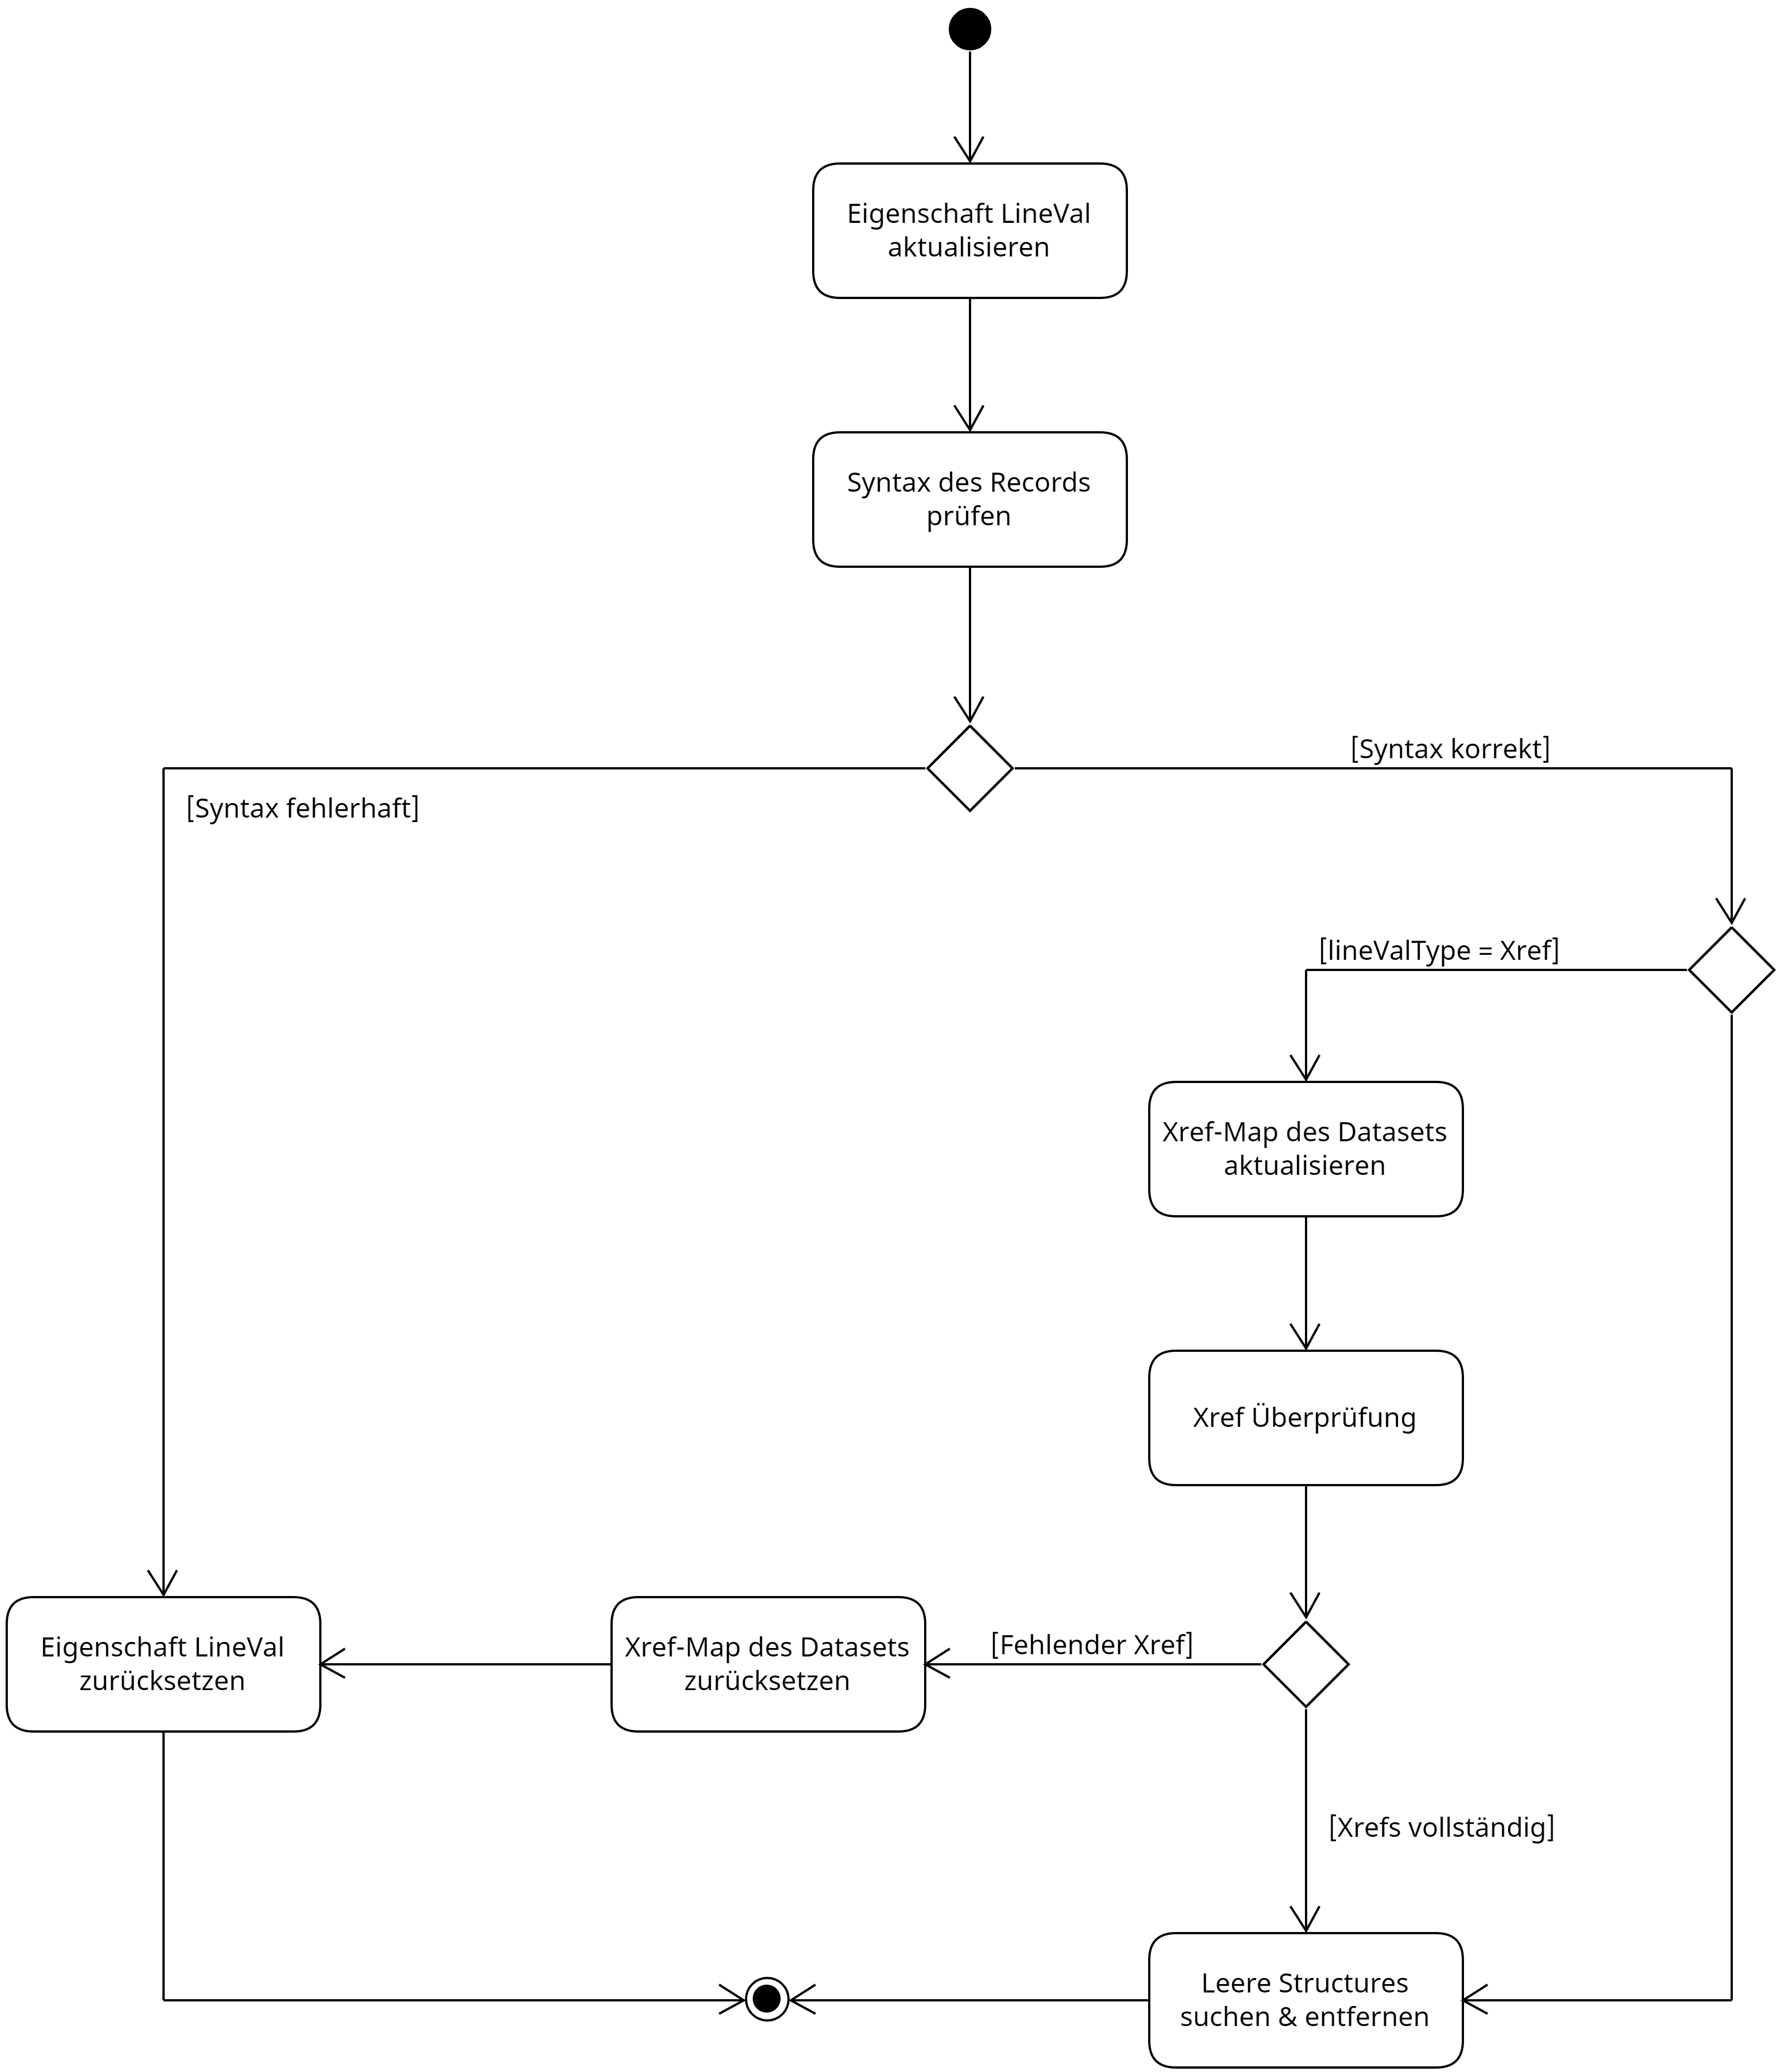
\includegraphics[width=0.5\textwidth]{images/UML_Activity_SetLineVal.png}
	\caption{UML Aktivitätsdiagramm der Methode \textit{setLineVal}}
	\label{fig: UML Aktivität setLineVal}
\end{figure}


\subsection{Klasse \textsc{Record}}
\label{subsec: Implementierung - Gedcom Struktur - Klasse Record}
Die Klasse \textsc{Record} ist die Vaterklasse für Family, Individual, Header, Multimedia, Repository, SharedNote, Source und Submitter und definiert eine Methode zur Syntaxüberprüfung eines Records. Dazu wird der entsprechende Nearley-Parser, der mit dem in Abschnitt \ref{sec: Implementierung - Grammatik Generator} beschriebenen \textsc{GrammarGenerator} erstellt wurde, eingebunden. Dieser bekommt alle Lines des Records kodiert als Zeichenkette als Eingabe und überprüft ob alle Structures syntaktisch korrekt sind.


Des Weiteren stellt die Klasse \textsc{Record} Methoden zur Verfügung, um Informationen aus Structures, die von mehreren Records geteilt werden, zu extrahieren und in gebündelter Form auszugeben. Ein Beispiel hierfür sind die Identifier-Structures, die genutzt werden um Structures oder ihre Inhalte eindeutig zu identifizieren. Die Klasse \textsc{Record} stellt dafür die Mehtode \textit{extractIdentifierStructures} zur Verfügung, mit der alle Identifier-Structures eines Records gesucht und in gebündelt zurückgegeben werden. Wie in Listing \ref{lst: extractIdentifier Funktion} dargestellt, wird die Methode \textit{getSubstructuresByUri} (siehe Abschnitt \ref{subsec: Implementierung - Gedcom Struktur - Klasse Structure}) verwendet, um alle Identifier-Structures des Records zu finden. Anschließend werden alle Informationen extrahiert und im JSON-Format zurückgegeben. 
\\ \\
\begin{minipage}{1.0\textwidth} \small
	\begin{lstlisting}
		  // extracts content of IDENTIFIER_STRUCTURE
		//  -> Each value provides an identifier for a structure or its subject, and each is different in purpose
		extractIdentifierStructures () {
			// REFN (Reference) is user-defined number or text that the submitter uses to identify the superstructure
			const references = this.getSubstructuresByUri('g7:REFN', false);
			
			// UID is a globally-unique identifier of the superstructure, to be preserved across edits
			const UIDs = this.getSubstructuresByUri('g7:UID', false);
			
			// EXID is an identifier maintained by an external authority that applies to the subject of the structure.
			const externalIdentifier = this.getSubstructuresByUri('g7:EXID', false);
			
			if (references || UIDs || externalIdentifier) {
				return {
					references: references?.map((ref) => {
						return {
							reference: ref.lineVal || null,
							type: ref.getSubstructuresByUri('g7:TYPE', false)[0]?.lineVal || null
						};
					}) || null,
					uniqueIdentifier: UIDs?.map((uid) => uid.lineVal),
					externalIdentifier: externalIdentifier?.map((exid) => {
						return {
							id: exid.lineVal || null,
							type: exid.getSubstructuresByUri('g7:EXID-TYPE', false)[0]?.lineVal || null
						};
					}) || null
				};
			}
			
			return null;
		}
	\end{lstlisting}
	\captionof{lstlisting}{Methode \textit{extractIdentifierStructures} der Klasse \textsc{Record}}
	\label{lst: extractIdentifier Funktion}
\end{minipage}
\\ \\

Alle Eigenschaften und Methoden der Klasse \textsc{Record} sind in Abbildung \ref{fig: UML Klassendiagramm Record} dargestellt.
\begin{figure}[h]
	\centering
	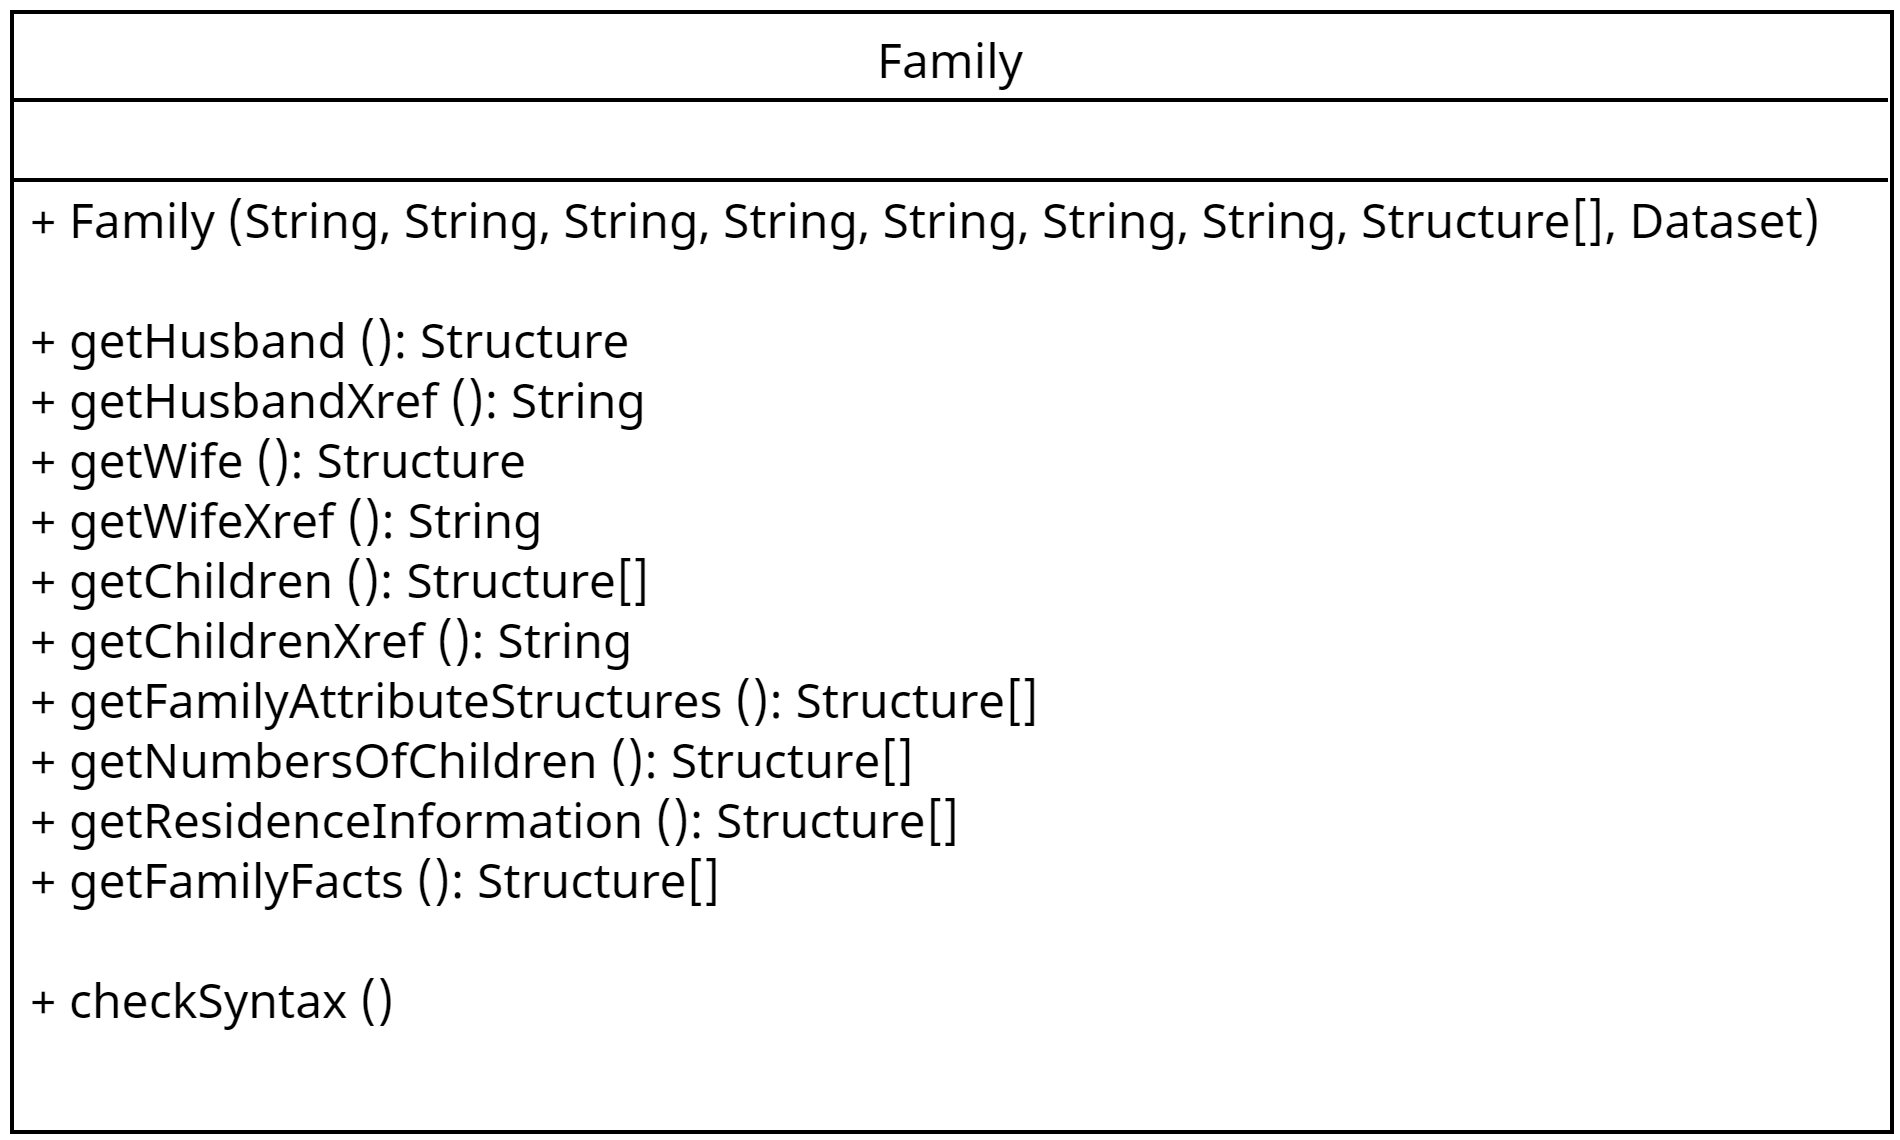
\includegraphics[width=1\textwidth]{images/UML_Class_Record.png}
	\caption{UML Klassendiagramm Record}
	\label{fig: UML Klassendiagramm Record}
\end{figure}

\subsection{Klasse \textsc{Family}}
Die Ziel bei der Erstellung der Bibliothek \textit{gedcom7.js} war es, eine Grundlage für die Verarbeitung von Gedcom7 Dateien zu kreieren, die in zukünftigen Arbeiten erweitert werden kann. Daher wurde für diese Arbeit nur die Klasse \textsc{Family} für den Family Record vollständig implementiert. Die Klassen für alle weiteren Records können analog zu dem hier beschrieben Vorgehen erstellt werden, um die Gedcom7 Spezifikation komplett abzubilden. 


Die Klasse \textsc{Family} ruft die Methode \textit{checkSyntax} der Vaterklasse \textsc{Record} mit der Family Grammatik auf. Des Weiteren werden Methoden zur einfachen Verarbeitung von Informationen aus einem Family Record bereitgestellt. Ist ein Anwender beispielsweise an Informationen über die Kinder einer Familie interessiert, müsste er die Gedcom7 Spezifikation studieren, alle Structures die Informationen über ein Kind bereithalten können nacheinander suchen und dann alle Informationen zusammenfügen. Um diese Arbeit zu erleichtern, werden in der Bibliothek \textit{gedcom7.js} die in Abbildung \ref{fig: UML Klassendiagramm Family} aufgeführten Convenience-Methoden bereitgestellt. Ein Beispiel hierfür ist die Methode \textit{getChildrenInformation}, mit der alle Informationen über die Kinder einer Familie extrahiert werden können:
\\ \\
\begin{minipage}{1.0\textwidth} \small
	\begin{lstlisting}
		 // returns information about the children of this family
		getChildrenInformation () {
			const famNCHI = this.getSubstructuresByUri('g7:FAM-NCHI', false)[0];
			const famEventDetail = this.extractFamilyEventDetail(famNCHI);
			
			if (famNCHI) {
				return {
					numberOfChildren: Number.parseInt(famNCHI.lineVal) || null,
					type: famNCHI.getSubstructuresByUri('g7:TYPE', false)[0]?.lineVal || null,
					parentInformation: famEventDetail?.parentInformation || null,
					eventDetails: famEventDetail?.eventDetails || null
				};
			}
			
			return null;
		}
	\end{lstlisting}
	\captionof{lstlisting}{Methode \textit{extractIdentifierStructures} der Klasse \textsc{Record}}
	\label{lst: extractIdentifier Funktion}
\end{minipage}
\\ \\
Dazu werden die entsprechenden Strukturen über die Methode \textit{getSubstructuresByUri} gesucht und im JSON-Format zurückgegeben. Alle Methoden und Eigenschaften der Klasse \textsc{Family} sind in Abbildung \ref{fig: UML Klassendiagramm Family} aufgeführt.

\label{subsec: Implementierung - Gedcom Struktur - Klasse Family}
\begin{figure}[h]
	\centering
	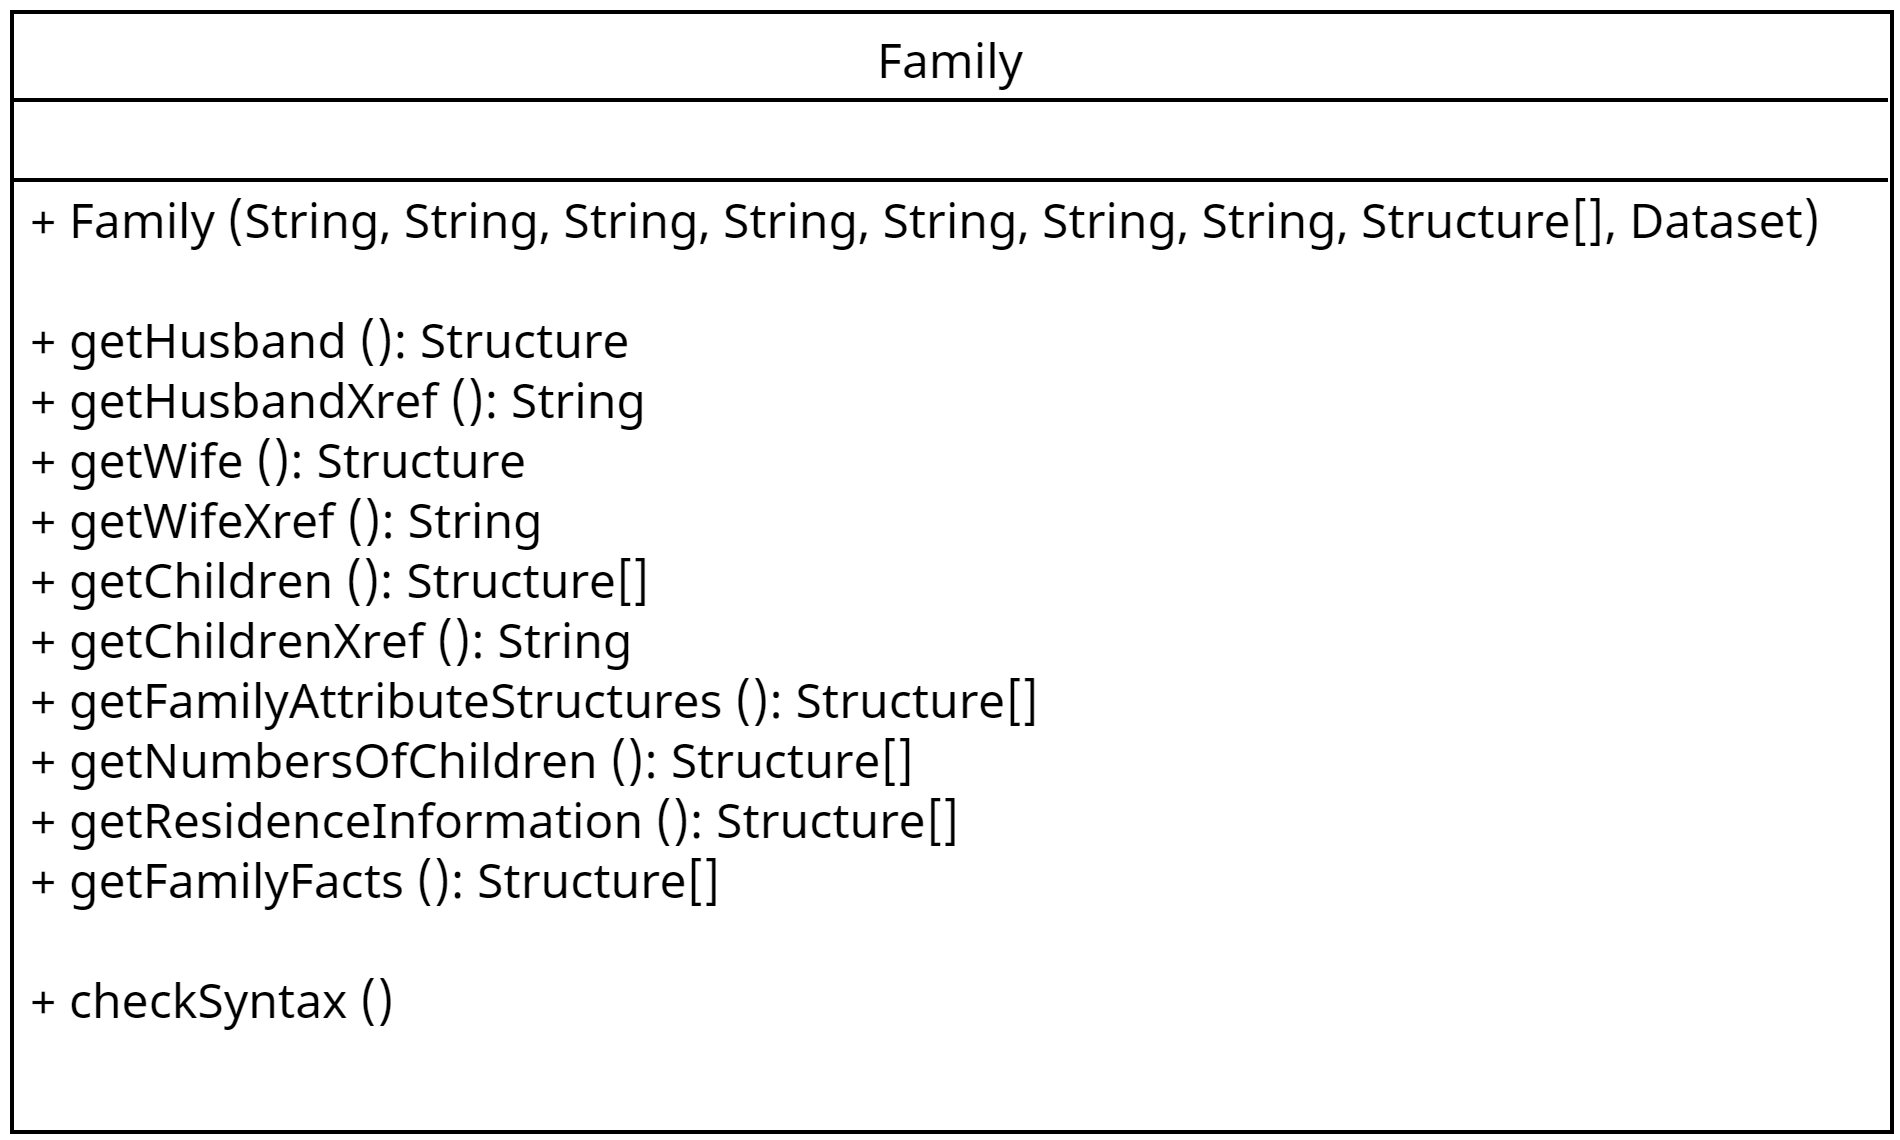
\includegraphics[width=1\textwidth]{images/UML_Class_Family.png}
	\caption{UML Klassendiagramm Family}
	\label{fig: UML Klassendiagramm Family}
\end{figure}

\subsection{Klasse \textsc{Dataset}}
\label{subsec: Implementierung - Gedcom Struktur - Klasse Dataset}
Die Hauptaufgabe der Klasse \textsc{Dataset} besteht darin, Structures zu erstellen und zu verwalten. Dazu werden die in Abbildung \ref{fig: UML Klassendiagramm Dataset} dargestellten Eigenschaften und Methoden verwendet. In den Eigenschaften jeder Instanz der Klasse \textsc{Dataset} werden Header und Trailer, alle Records die enthalten sind, Datenstrukturen zur Verwaltung von Cross-Reference-Identifiern, sowie Informationen über die Verwendung des Byte-Order-Mark und End-Of-Line Characters gespeichert. Bei der Erstellung einer Instanzt der Klasse \textsc{Dataset} über den Konstruktor können Header-, Trailer- und Record Informationen übergeben werden, aus denen Instanzen der Klasse \textsc{Structure}, bzw. \textsc{Record} generiert werden. Zudem kann ein leeres Dataset über die Methode \textit{createEmptyDataset} erstellt werden.\\
Die Klasse \textsc{Dataset} übernimmt vier Aufgaben: 

\vspace{1em}
\textbf{1. Erstellen von Structures} \vspace{0.5em} \\
Mit Hilfe der Methode \textit{createStructure} können Structures auf Basis von Informationen, die vom Nearley Parser zurückgegeben wurden, erstellt werden. Zusätzlich werden Informationen zur Superstructure und dem Record zu dem die Structure gehört, benötigt. Auf Basis dieser Informationen kann die passende Structure erstellt werden, Referenzen andere Structures angepasst und bei Bedarf Einträge in die Xref-Map erstellt werden. 

\vspace{1em}
\textbf{2. Hinzufügen/Entfernen von Records} \vspace{0.5em} \\
Die Methoden \textit{addRecord} kann verwendet werden um neue Records auf Basis von übergebenen Structure Informationen zu erstellen und ins Dataset einzugliedern. Benötigt werden dazu die Gedcom7 URI, der LineValue (sofern dieser vorhanden ist) und die Substructures, die enthalten sein sollen. Anschließend werden die Referenzen im Dataset so angepasst, dass der Record an der richtigen Stelle eingeliedert wird.


Mit \textit{removeRecord} kann ein Record mit der gegebenen Referenz aus dem Dataset entfernt werden. Dabei wird der Eintrag aus der Xref-Map entfernt. Außerdem wird überprüft, ob eine Structure im Dataset über einen Cross-Reference-Identifier auf den entfernten Record verweist. Wenn dies der Fall ist, muss die entsprechende Referenz zu einem @VOID@-Pointer geändert werden, da nicht auf nicht-definierte Xrefs verwiesen werden darf \cite{GEDCOM}. Zusätzlich wird eine Warnung für den Benutzer ausgegeben um darauf hinzuweisen, dass das Entfernen eines Records dazu führt, dass ebenfalls alle Substructures entfernt werden. 


\vspace{1em}
\textbf{3. Hinzufügen/Entfernen von Structures} \vspace{0.5em} \\
Mit den gleichen Informationen wie beim Hinzufügen von Records, können auch Structures zum Dataset hinzugefügt werden. Zusätzlich werden die Superstructure und der Record benötigt, in den die Structure eingefügt werden soll, um ein richtiges Eingliedern ins Dataset zu ermöglichen. 


Die Methode \textit{removeStructure} kann verwendet werden, um Structures aus dem Dataset zu entfernen. Hierbei sind im Gegensatz zum Entfernen von Records weitere Überprüfungen notwendig. Wenn das Entfernen einer Structure dazu führt, dass die Superstructure weder einen LineValue, noch Substructures hat, sollte die Superstructure ebenfalls entfernt werden \cite{GEDCOM}. Außerdem kann das Entfernen einer Structure dazu führen, dass die Syntax der Superstructure nicht mehr korrekt ist, z.B. weil die Structure in der Gedcom7 Spezifikation als erforderlich (Kardinalität 1:1 oder 1:M) definiert wurde. In diesem Fall wird die Structure beibehalten und ein dem Datentyp entsprechender Leerer Wert wird als LineValue eingetragen \cite{GEDCOM}. Auch hier wird eine Warnung für den Benutzer ausgegeben um darauf hinzuweisen, dass das Entfernen eines Records dazu führt, dass ebenfalls alle Substructures entfernt werden. 

\vspace{1em}
\textbf{4. Suchen von Record} \vspace{0.5em} \\
Die Klasse \textsc{Dataset} implementiert verschieden Methoden um Records im Dataset zu suchen. Beispielsweise können über die Methode \textit{getFamilyRecords} alle Family Records des Datasets zurückgegeben werden. Sucht man einen bestimmten Record, kann dieser über \textit{getRecordByXref} über den Cross-Reference-Identifier gefunden werden. 

\vspace{1em}
\textbf{5. Ausgabe als Gedcom7 konformer String} \vspace{0.5em} \\
Eine wichtige Anforderung für die Bibliothek \textit{gedcom7.js} war es, dass die eingelesenen Gedcom7 Dateien wiederausgegeben werden können. Dazu implementiert die Klasse \textsc{Dataset} die Methode \textit{toString}. In dieser Methode werden für alle Records, Header und Trailer die \textit{toString} Methode aufgerufen, die in der Klasse Structure so definiert ist, dass alle Structure-Informationen in Form einer Gedcom7-konforme Line zurückgegeben werden. Diese Lines werden in der richtigen Reihenfolge zusammengehangen und ergeben so eine Zeichenkette, die mit Hilfe der asynchronen Methode \textit{write} am spezifizierten Pfad in Form einer Gedcom7 Datei gespeichert werden kann.

\begin{figure}[h]
	\centering
	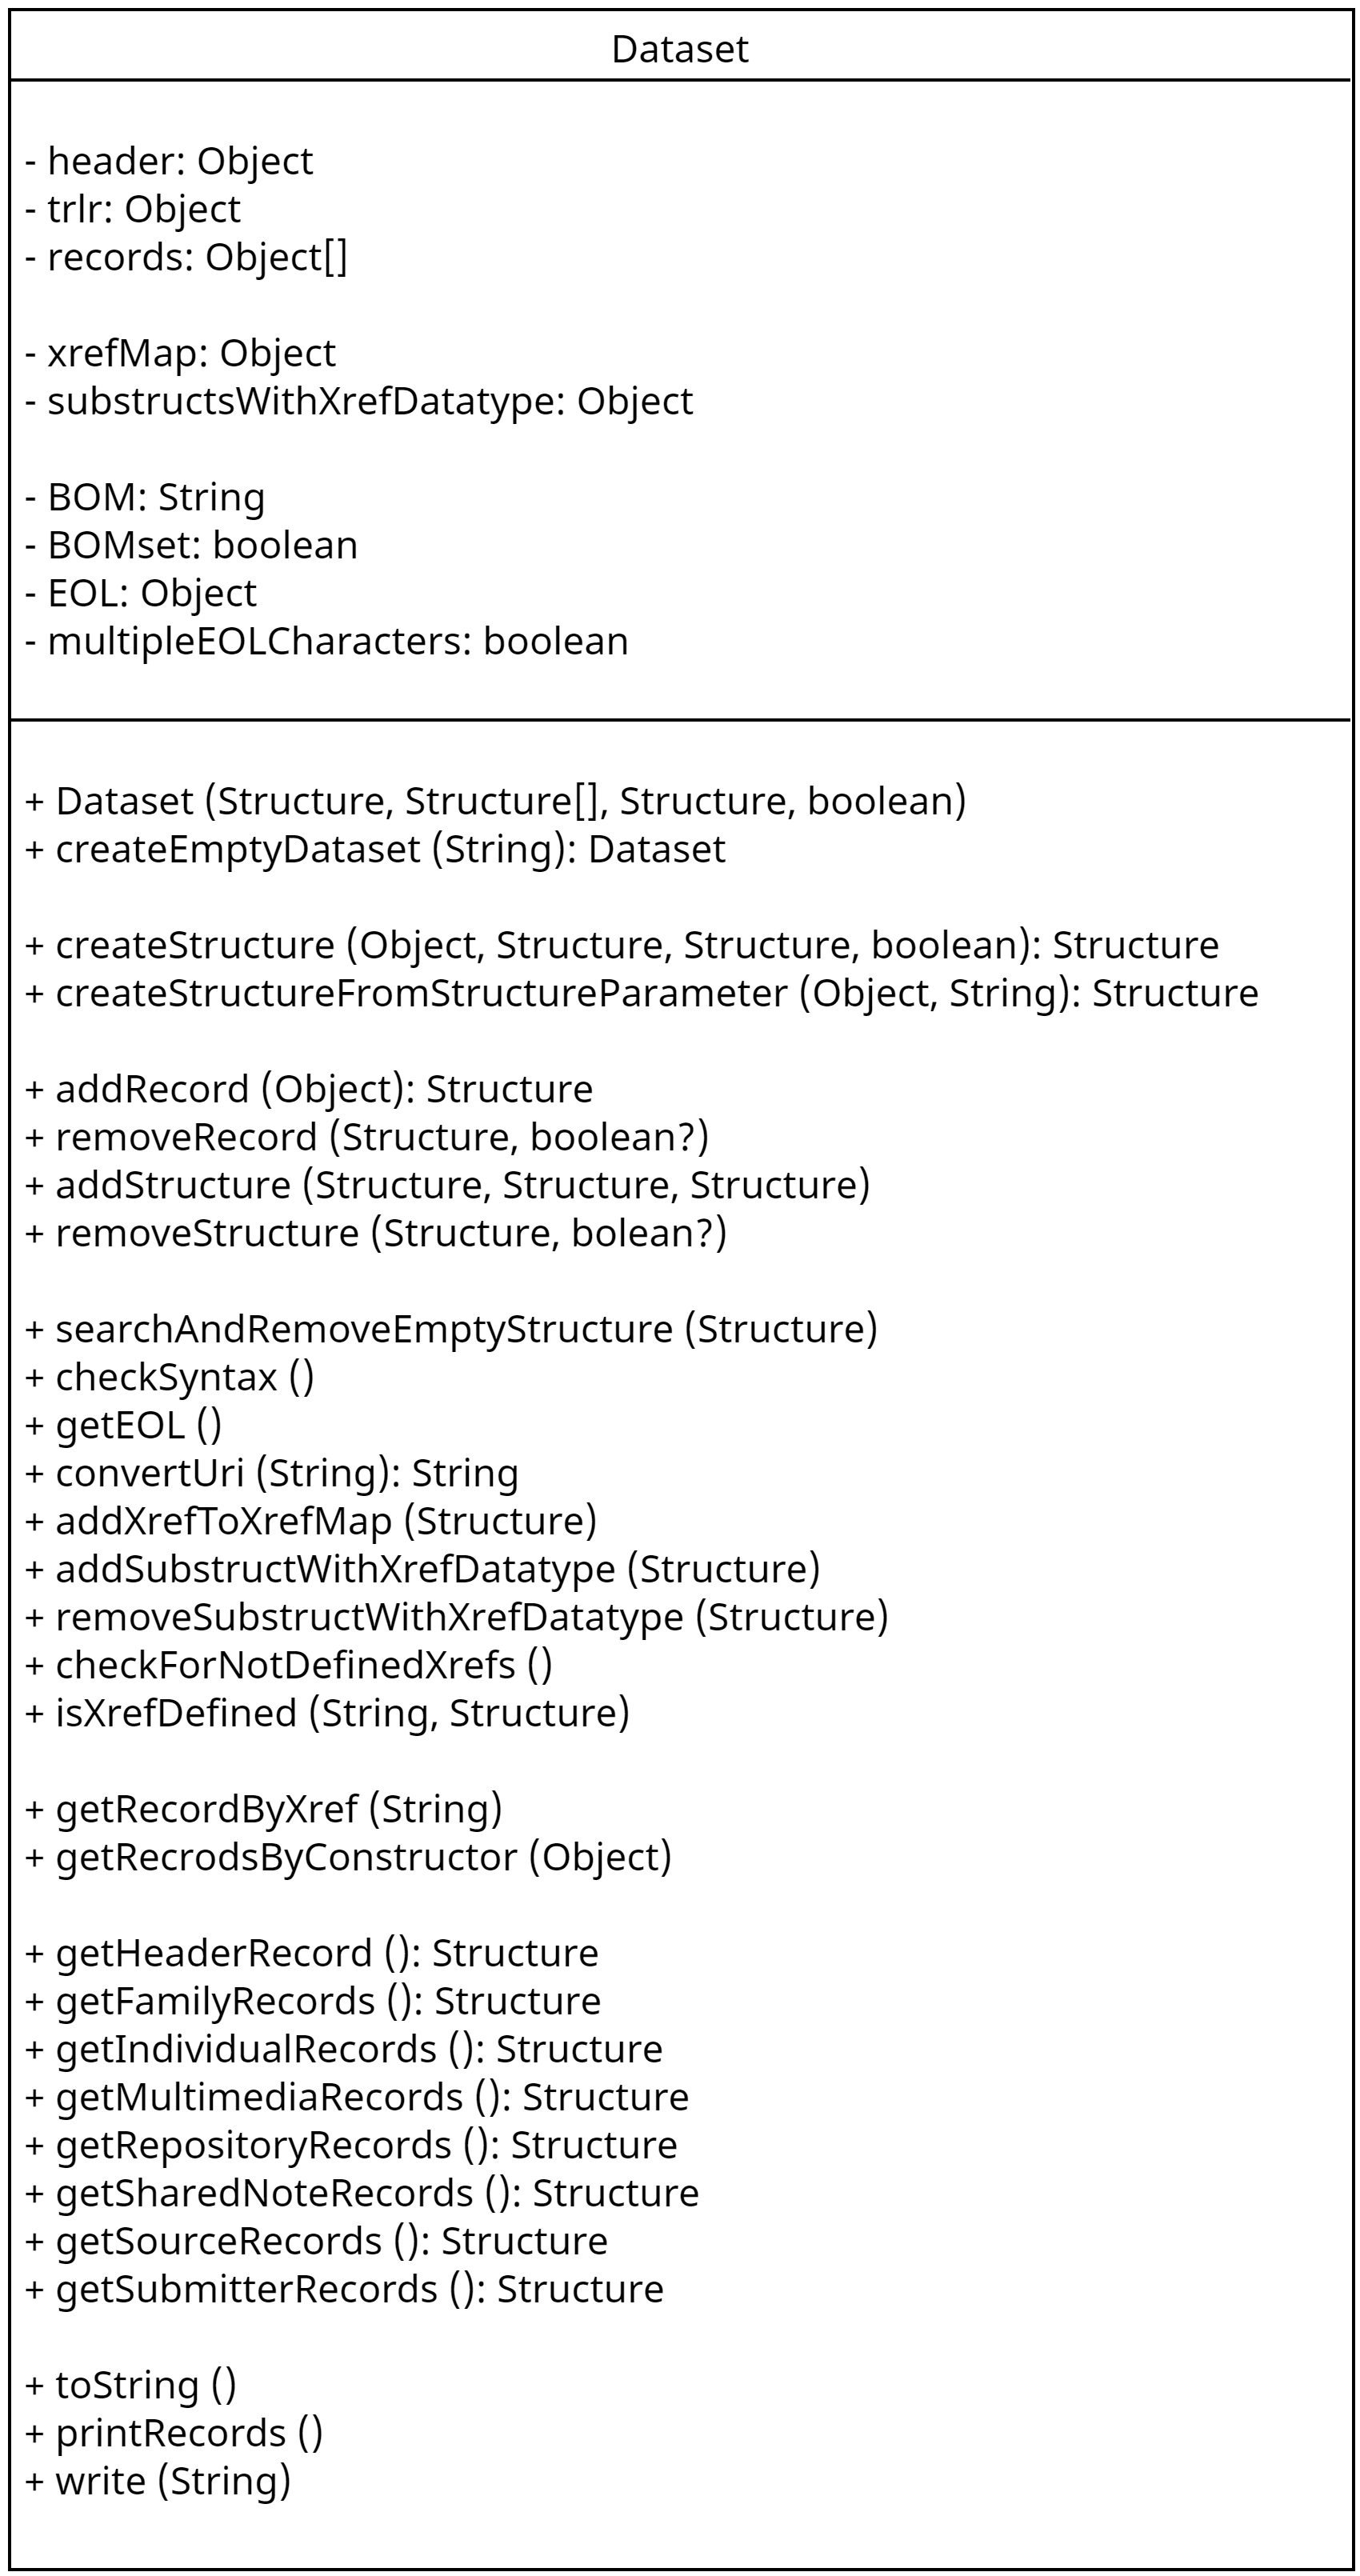
\includegraphics[width=0.65\textwidth]{images/UML_Class_Dataset.png}
	\caption{UML Klassendiagramm Dataset}
	\label{fig: UML Klassendiagramm Dataset}
\end{figure}


%========================================================================================
% SECTION: GEDCOM Parser
%========================================================================================
\section{Gedcom Parser}
\label{sec: Implementierung - Gedcom Parser}
Alle in dieser Arbeit vorgestellten Konzepte und Implementierungen werden im \textsc{Gedcom Parser} vereinigt, der die zentrale Klasse der Bibliothek \textit{gedcom7.js} darstellt. Die Klasse \textsc{GedcomParser} verfügt über die Methode \textit{parseGedFile} mit der Gedcom7 Dateien mit Hilfe der Node.js FileSystem Bibliothek als UTF-8 kodierte Zeichenkette eingelesen und anschließend mit der Methode \textit{parseString} geparsed werden kann. Wie im Konzept in Abschnitt \ref{sec: Konzept - Gedcom Parser} dargestellt, wird ein Nearley Parser erstellt für ein Dataset erstellt, der String geparsed und anschließend aus den extrahierten Informationen eine Instanz der Klasse \textsc{Dataset} erzeugt die zurückgegeben wird. Das Sequenzdiagramm dieser Methode ist in Abbildung \ref{fig: Sequenz Gedcom Parser} dargestellt. \\
Im folgenden wird ein beispielhafter Ablauf für die Verwendung der Bibliothek \textit{gedcom7.js} dargestellt. Dazu wird eine Gedcom7 Datei eingelesen, die den FamilyRecord aus Listing \ref{lst: family record example} enthält:\\
Im ersten Schritt wird die Gedcom7 Datei eingelesen, geparsed und in ein Dataset überführt. Dazu wird eine Instanz der Klasse \textsc{GedcomParser} erzeugt.
\begin{center}
	gedcomParser = new GedcomParser();
\end{center}
Anschließend wird der Pfad zur Gedcom7 Datei an die Methode \textit{parseGedFile} übergeben. In diesem Beispiel liegt die Datei im selben Verzeichnis, wie die ausgeführte JavaScript-Datei unter dem Namen ''FamilyExample.ged``. 
\begin{center}
	const dataset = await gedcomParser.parseGedFile('./FamilyExample.ged');
\end{center}
Dann kann die Family aus Listing \ref{lst: family record example} über den Cross-Reference-Identifier gesucht werden.
\begin{center}
	const famF1 = dataset.getRecordByXref('@F1@');
\end{center}
Sollen Informationen über die Kinder der Family ausgegeben werden, kann dies über 
\begin{center}
	const nchi = famF1.getChildrenInformation();
	console.log(nchi);
	// Ausgabe: 
	// {
	//    numberOfChildren: 2,
	//	  type: null,
	//    parentInformation: null,
	//    eventDetails: null
	// }
\end{center}
realisiert werden. Außerdem kann Datum der Hochzeit herausgefunden werden, kann dies folgendermaßen aussehen:
\begin{center}
	const marrInfo = famF1.getMarriageInformation();
	console.log(marrInfo.marriages[0].eventDetails.date);
	// Ausgabe: 
	// {
	//    type: "DateValue"
	//    date: 1951-03-01T00:00:00.000TZ
	// }
\end{center}
Soll nun die Information zum Family Record hinzugefügt werden, dass die Ehe wieder geschieden wurde, kann dies über die DIV-Structure ausgedrückt werden. Mit Hilfe der Methode \textit{addSubstructure} kann eine DIV-Structure zum Family Record hinzugefügt werden:
\begin{center}
	const div = {
		uri: 'g7:DIV',
		substructs: [{
			uri: 'g7:DATE',
			lineVal: '28 DEC 1963',
		}]
	};
	famF1.addSubstructure(div);
\end{center}
Wird der Family Record nun ausgegeben, ist die neue DIV-Structure in der Ausgabe mit korrekter Gedcom7 Line-Syntax enthalten:
\begin{center}
	console.log(famF1.toString());
	// Ausgabe: 
	// 0 @F1@ FAM
	// 1 HUSB @I1@
	// 1 WIFE @I2@
	// 1 MARR
	// 2 DATE 1 MAR 1951
	// 1 NCHI 2
	// 1 DIV
	// 2 DATE 28 DEC 1963
\end{center}
